

\chapter{Guide path: LEAS}
\label{sec:LEAS}
\minitoc
\bigskip

%\textcolor{blue}{A REVOIR MAINTENANT COMME ON A ECRIT LA SOTA + INTRO}
In this chapter, we present our method to Learn To Steer a locomotion contact planner \qq{LEAS}, the core module of this thesis. 
Our steering method answers the question: \textit{How to locally navigate complex and unknown terrains subject to validity and collision constraints?}
% Input / Output
LEAS takes as input a desired direction and a local height map of its surrounding terrain, to generate a robot root trajectory.
As many solutions exist to solve such a task, we provide an insight into our design choices and particularly why we use Reinforcement Learning.

In this section, we focus on the implementation of LEAS, which will be reused and adapted for different contact planners through Chapters \ref{sec:CP-SB} and \ref{sec:CP-SL1M}.

This chapter is organized as follows: 
In Section \ref{subsec:leas-motivation} we describe the context and the challenges we want to solve. In Section \ref{subsec:leas-RL} we present the specification of the problem and our solution LEAS \cite{LEAS}. We describe it as an RL agent and explain our design choices for its observation, control, and reward to achieve the desired navigation behavior.
In section \ref{subsec:leas-implementation}, we present our implementation regarding the feasibility approximations, the random terrain generation, and the learning architecture.
%additional libraries implemented to optimize the computation time and to create random terrains where to train and evaluate our steering method.
In Section \ref{subsec:leas-results}, we evaluate how LEAS can navigate unknown terrains under reachability and collision avoidance constraints, and compare its results to some other model-based steering methods.
Finally, we discuss the advantages, limitations, and potential improvements of our local navigation method.

\section{Motivation\label{subsec:leas-motivation}}
\subsection{Context\label{subsubsec:context}}

\begin{figure}[h!]
    \centering
    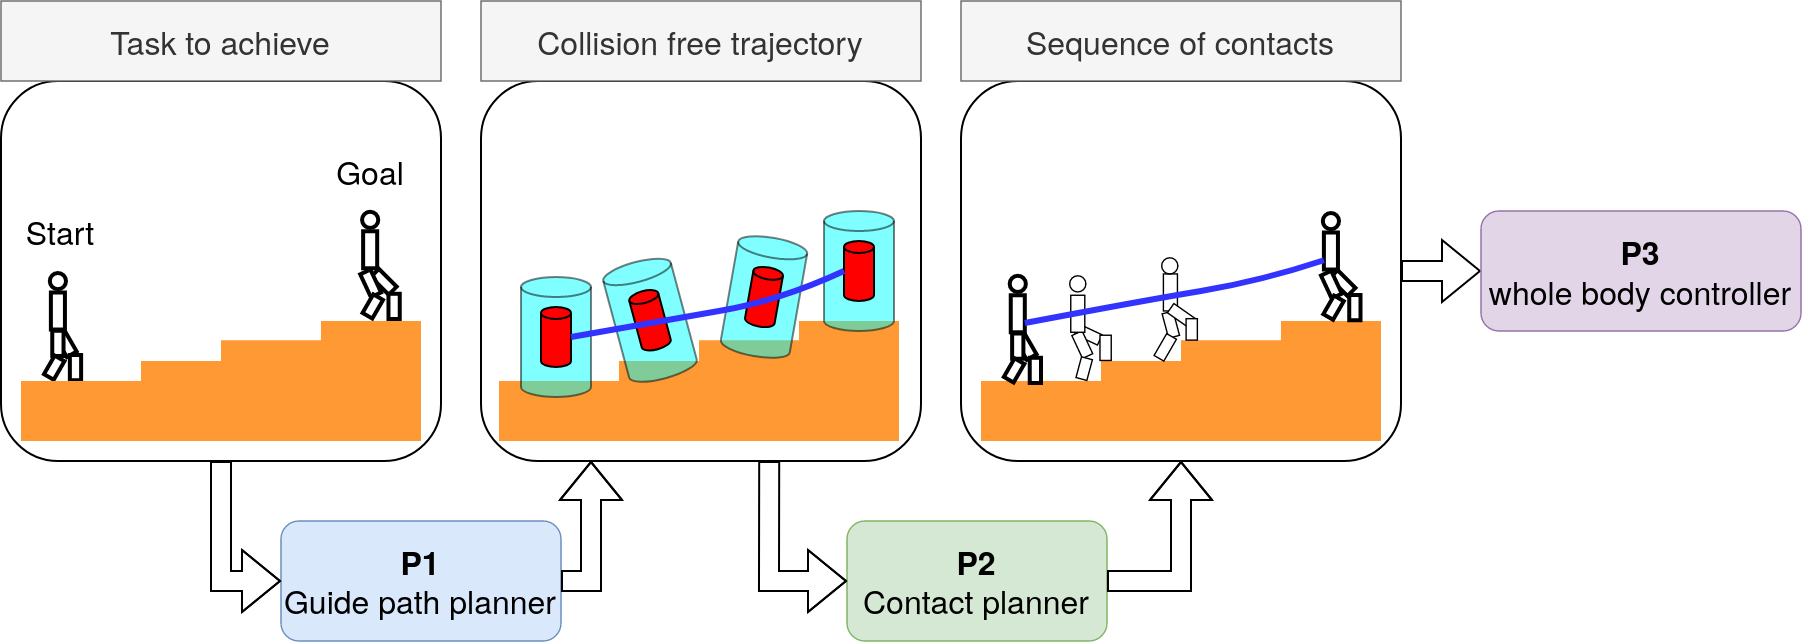
\includegraphics[width=\textwidth]{Figures/Chapter_LEAS/pipeline.png}
    \caption{Pipeline of the Loco3D project addressing the locomotion with a multi-stage approach.}
    \label{fig:pipeline}
\end{figure}


% Re-explain all the context with the division of the locomotion into three phases: Guide path planning - Contact planning - Whole body locomotion.
%In this work, we place ourself in a multi-stage framework \cite{loco3d} that divides the locomotion problem into three sub-tasks as shown on Figure \ref{fig:pipeline}: first \stn{c est quoi p1 ? definis. tu devrais dire que chaque p est un probleme} $P1$ generates a root trajectory, also referred as \qq{guide path}, then $P2$ generates a sequence of contacts on this guide, and finally $P3$ performs these contacts with a whole body controller on the robot.
As discussed in the previous chapter, the most recent locomotion planners are structured in several hierarchical stages. Let us now present in detail how we structured our planner, based on the seminal work that drives the locomotion methodology in our team \cite{loco3d}.
The general organization is shown in Figure \ref{fig:pipeline}.

% All pipeline
The first stage generates a \textit{guide path} ($P1$), i.e. a trajectory in translation and rotation that we would like to follow with the main robot body, referred to as the \textit{root} (i.e. the basis of the torso for Talos). In the second stage, a contact planner ($P2$) computes the contacts along the guide path. In the last stage, a whole-body controller ($P3$) computes the control sent to the robot to perform these contacts.

% What we opt for: motion-before-contact
The decoupling of $P1$ and $P2$ has proven successful in \cite{Escande2008Guide, bouyarmane2009} and later on in \cite{loco3d, RB-PRM}, where each sub-task can be solved independently from each other, thus reducing the complexity of the problem and allowing us to experiment and compare different module implementations. 
%\stn{il manque le papier de bretl, relis bien mon eta tde l art de these pour avoir lhistorique}
%\textcolor{blue}{answer: Bretl and Hauser are contact-before-motion, they will be already cited in the SOTA.}

% Guide path definition
The first module $P1$ generates a guide path, defined in this thesis as a discrete sequence of configurations for the robot root in $SE(3)$ (i.e. position and orientation).
% Division strategy of path planning
This navigation module can be further divided into two parts: a Steering Method (SM) and a path planning algorithm.
The SM locally navigates the terrain following a given direction, while path planning uses the SM to sequentially reach sub-goals (also called waypoints) up to a distant objective. 
On the resulting guide path, all configurations must respect two constraints as expressed in \cite{RB-PRM} and shown in figure \ref{fig:ROMs}.
%\stn{ça va bien trop vite àa. C est un point important et differentiant. tu dois expliquer comment on fait du sampling based serieusement ici}
%\textcolor{blue}{answer: Sampling-based for path planning you mean? Already done in the SOTA in the path planning section (but briefly). A REVOIR APRES L'ECRITURE DE LA SOTA.}

\begin{figure}
    \centering
    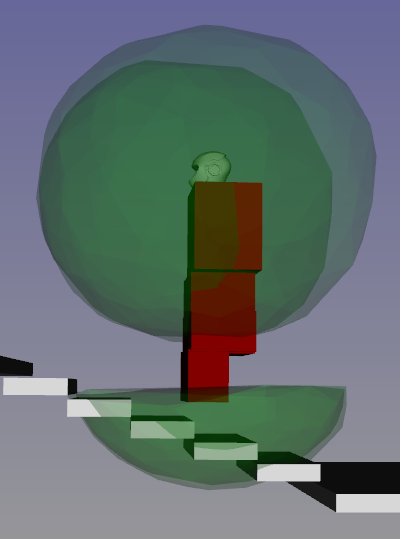
\includegraphics[width=0.3\textwidth]{Figures/Chapter_LEAS/ROMs.png}
    \caption{Validity constraints of the Talos Robot, (green) ranges of motion of each end effector, and (red) the robot trunk. The configuration above is valid as the robot can potentially reach the ground ($\mathcal{R}$) and the trunk is not in collision with the terrain ($\mathcal{C}$).}
    \label{fig:ROMs}
\end{figure}

The first constraint $\mathcal{R}$ is referred to as the \textit{reachability} and imposes that the robot, at a given root configuration, has a non-null contact reachable space (i.e must be able to touch the ground). 
This constraint is approximated as a reachability volume, which is a polytope representing the range of motion of one effector of the robot.
As long as an intersection exists between the terrain and the reachability volume for a given configuration, we consider that this constraint is respected.
For simplicity's sake, we consider in this thesis only one reachability volume as the union of both legs polytopes.
The second constraint $\mathcal{C}$ is referred to as \textit{collision avoidance} and imposes that the robot must not be in contact with the terrain other than with its end effectors (foot and hands). This constraint is approximated as a polytope representing the robot trunk. If an intersection exists between this polytope and the terrain, the configuration is considered in collision.
In this manuscript, we will consider a configuration as valid if it respects both constraints $\mathcal{R}$ and $\mathcal{C}$, that approximate the feasibility of the problem by the next module (the contact planner).
% Steering methods at our disposal in Loco3D
We have two Steering Methods at our disposal in \cite{loco3d}:
\begin{itemize}
    \item RB-Lin, a linear interpolation between two configurations in $SE(3)$. In all our scenarios, we program RB-Lin to first interpolate on the orientation, i.e. to rotate the robot toward the goal with the angular velocity $\omega_{max}$, then to interpolate on the position by moving the robot at $v_{desired}$ each timestep $T$ until reaching the goal;
    \item RB-Kino \cite{kinodynamic_sm_2017}, which uses a Double-Integrator Minimum-Time control \cite{DIMT}, is a kinodynamic SM connecting exactly two configurations in position, velocity, acceleration, and orientation.
\end{itemize}
The main limitation of these SM is that they do not consider collisions and reachability with the terrain, therefore relying on path planning to validate these constraints along the trajectory.
In this work, we will either manually give the sequence of waypoints to reach, or use a reachability-based probabilistic roadmap \cite{RB-PRM} as a path planning algorithm with these model-based methods. 
% Explanation of steve algo (not my work so I won't go too much into it?)
%Its concept is to generate candidate configurations by translating and rotating the robot root by a small increment until $\mathcal{C}$ and $\mathcal{R}$ can be met (full algorithm and details in \cite{thesis_steve}).
%\stn{pareil ici c est complique, juste redonne l algo prm en fait et tu peux repartir de la apres. Il fait 10 lignes et tu peux le copier direct de ma these}
%\textcolor{blue}{answer: Je l'ai vite fait mis dans la sota, et je ne l'utilise pas vraiment donc ce n'est peut etre pas utile de le dire. J'ai juste renvoyé vers ta these.}

\begin{figure}
    \captionsetup[subfigure]{justification=centering}
    %\centering
    \begin{subfigure}[t]{.49\linewidth}
    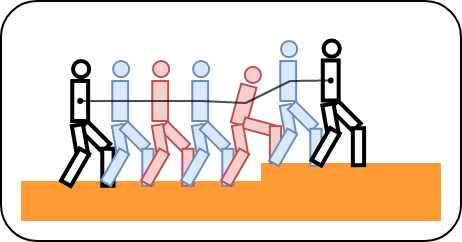
\includegraphics[width=\textwidth]{Figures/Chapter_LEAS/strategies_cp_guide_A.png}
    \caption{Find key contact configurations along the root trajectory\label{fig:strategies_cp_acyclic}}
    \end{subfigure}
    \begin{subfigure}[t]{.49\linewidth}
    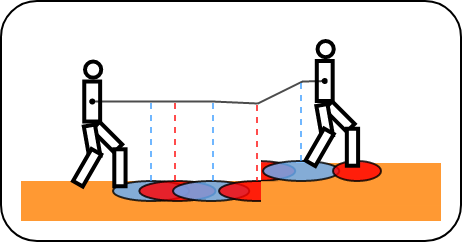
\includegraphics[width=\textwidth]{Figures/Chapter_LEAS/strategies_cp_guide_B.png}
    \caption{Solve the surface selection problem for all steps\label{fig:strategies_cp_mip}}
    \end{subfigure}
    \caption{Contact planner strategies, (a) generates key configurations contact following the root trajectory in input, (b) discretizes the guide to find potential surfaces to step on.}
    \label{fig:strategies_cp}
\end{figure}

The second module $P2$ receives a guide path as input and populates it with a contact sequence. Such a contact planner can have different strategies on how to use the guide. In this thesis, we will explore two strategies for quasi-static contact planning with very distinct problem formulations. 
% Acyclic
The first uses the guide path directly as an exact root trajectory to follow and computes the contacts along it (Figure \ref{fig:strategies_cp_acyclic}).
%The contact planner used in chapter \ref{sec:CP-SB} follows this strategy.
% MIP
The second uses the guide to get some candidate surfaces to step on, then solves a surface selection problem to have exactly one surface selected for each contact (Figure \ref{fig:strategies_cp_mip}).
% Why this decomposition, benefits
The decomposition of the contact planning problem in P1 and P2 (motion-before-contact) breaks the algorithm complexity \cite{AcyclicCP,sl1m_v2} of the contact planning problem, by constraining the search for contacts in the guide path vicinity.

Lastly, the module $P3$ performs the contact sequence on the robot with a whole body controller \cite{loco3d, tsid_prete, deepLoco}. For future work, we also implemented an environment to learn such a whole-body controller via deep RL \cite{software_robot_RL}.
In this thesis, we will not use the module $P3$ and focus on the contact planning problem ($P_1$ and $P_2$).


\subsection{Problem Statement\label{subsub:problematic_leas}}

% Motivation
In this context of division into two independent sub-tasks $P1$ and $P2$, the price to pay for the simplification of the contact planning problem is the absence of guarantees of feasibility between the different modules.
In such a sequential framework, the success of a module is a necessary condition for the success of the next in the pipeline but not sufficient.

That is why some approximations are required to increase the feasibility of the next module, such as the reachability condition $\mathcal{R}$ in $P1$. The guide path planner assumes that if the ground is reachable at all times along the path, then it is possible to generate a contact sequence. 
This strategy has been proven effective in many scenarios \cite{AcyclicCP}, but can still fail as we will see in the next chapters, weakly approximating the capabilities of the contact planner plugged in. Each contact planner behaves differently as seen in Figure \ref{fig:strategies_cp} and we do not know what makes a feasible guide path for it. As a consequence, it is difficult to define new additional constraints or heuristics in our navigation module ($P1$) to better approximate the contact planning feasibility ($P2$).

% Given the previous context, what do we want ?
We want to fix this issue with a high-level approach, on the very first module of the pipeline $P1$.
The problem we are trying to solve can be formulated as the question: \textit{What is a feasible guide path for a given contact planner ?} 
In other words, how can we build a guide path planner that will better approximate the feasibility space of the contact planner. Such a planner could improve the success rate of $P2$ and sequentially, the success of the whole pipeline.

% Why do we focus on the steering method
As explained previously, $P1$ can be decomposed into two components: a path planning algorithm generating some waypoints to reach, and the SM that sequentially connects these waypoints.
In this thesis, we focus on the steering method that locally generates a guide path between two waypoints.
We want to build an SM able to locally navigate while observing the surrounding terrain to avoid obstacles and validate the reachability condition. 

% Why not working also on path planning ?
% If we have a good SM, then it makes the control a lot more easier for path planning algorithm.
% Path planning algorithm uses the SM to define control points (waypoints) to reach an objective. The SM returns if it succeeded or not to reach this waypoint. A too simple steering method unable to grasp the complexity of the terrain will have a lot of troubles to follow far away waypoints and will makes the search very difficult for the path planning algorithm, requiring more 
The reason why we do not further investigate path planning in this work is that in most simple scenarios, such as walking on flat ground or climbing some stairs, a steering method should be enough to generate a valid trajectory. Doing so also removes the need for a path planning algorithm (RRT, PRM) expensive to compute.
%In the future, the implementation of more efficient path planning algorithm as \cite{RL_RRT} will be implemented.

% What's our solution and why do we use RL for that ?
We build such a terrain-aware steering method with deep Reinforcement Learning (RL).
The choice of using RL is motivated by its capabilities to learn a representation of its environment and to act in it, while maximizing the future cumulative reward and keeping a valid state.
An SM learned by reinforcement could learn how to navigate locally with a vision of its surrounding terrain, while respecting the validity constraints ($\mathcal{R}$ and $\mathcal{C}$) and increasing the success rate of the contact planner.

In this chapter, we first train a pure steering method and provide the results. 
In the next chapters, we use a contact planner as an oracle to validate the trajectories during the learning, then we observe what behavior changes on the SM to increase its success rate.


\section{LEAS: an RL Steering Method\label{subsec:leas-RL}}
% What behaviour do we want for the SM ?
Given initial and goal configurations, we learn by reinforcement a steering method generating a guide path in a given direction while respecting both reachability and collision constraints ($\mathcal{R}$ and $\mathcal{C}$). 
To that end, we designed LEAS \cite{LEAS}, an RL agent that learns by trial and error how to perform this task and to generalize to unknown environments. An overview of our method is presented in figure \ref{fig:LEAS}. The main idea behind LEAS is that for each action taken in the environment, the configuration in $SE(3)$ of the robot will be modified and stored in a list: the guide path.

\begin{figure}
    \centering
    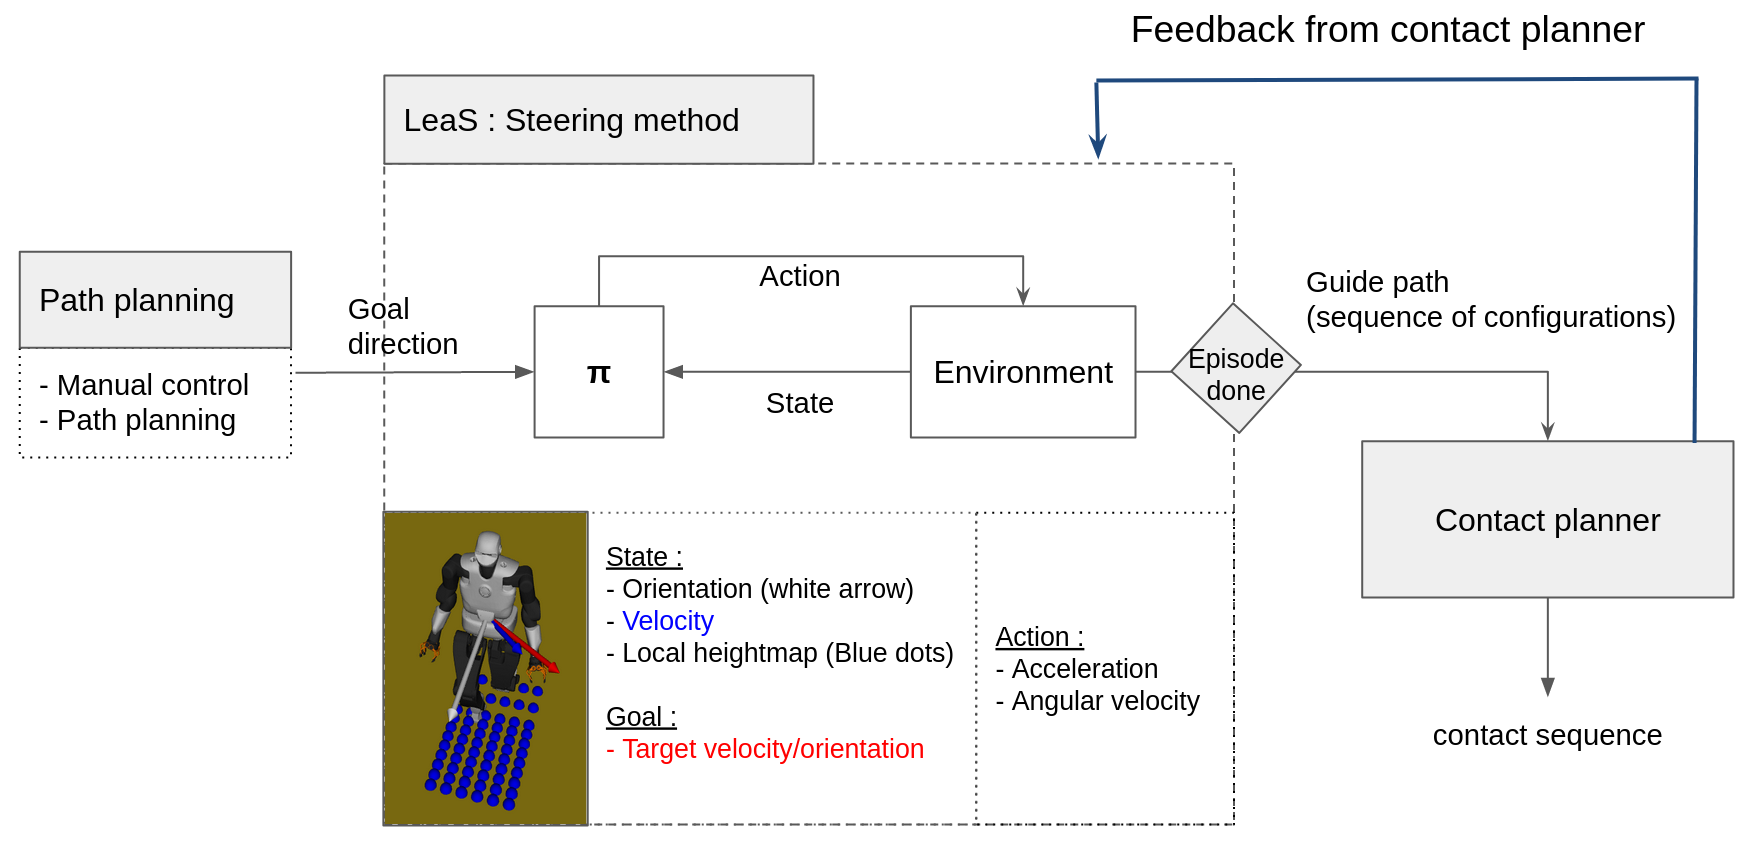
\includegraphics[width=\textwidth]{Figures/Chapter_LEAS/leas_overview.png}
    \caption{Overview of LEAS: the user or a path planning algorithm inputs a target direction to our steering method. LEAS is an RL agent that moves the robot in the environment and sequentially saves all its states. Once the episode is over, this state sequence is the guide path given to the contact planner $P2$. Finally, $P2$ returns an evaluation of the contact plan success that makes LEAS learn how to generate feasible guide paths for it.}
    \label{fig:LEAS}
\end{figure}

In this section, we will take a look at the result of LEAS without plugging it to a contact planner.
Explanations on how LEAS can improve the success rate of a given contact planner will be left for chapters \ref{sec:CP-SB} and \ref{sec:CP-SL1M}.

\subsection{Specifications \label{subsubsec:specifications}}
% What behaviour do we want LEAS to have.
% Goes in depth point by point on every specification of the first sentence, translating it into RL actions/states etc.
We need to specify the task we want to perform with LEAS, with what behavior, and how to achieve it with Reinforcement Learning.

We choose to input a goal direction in LEAS instead of a goal configuration.
We defined a steering method as a planner following a rough path, hence generating a trajectory ending closer to the goal than initially, and that is exactly what LEAS does by moving in the goal direction.
This input also allows for more flexible user controls that can set a fixed goal (reachable or not) in the environment or steer in a direction with a joypad.

Following this design, we desire LEAS to have the following list of behaviours:
\begin{enumerate}[label=(\Alph*)]
  \item Move in the goal direction at a fixed desired velocity.
  \item Respect the reachability and collision constraints, $\mathcal{R}$ and $\mathcal{C}$. 
  \item Stop if it can not go further (i.e keep a valid state).
  \item Navigate locally without the help of path planning, meaning that LEAS should only act based on a very short vision range.
  \item Orientate its root in the desired goal direction. This design choice can be limiting in cluttered environments where side walking is required, but was necessary for our experiments to obtain a straight walk (sidewalking was a predominant locomotion strategy without this specification, as we will discuss in the next chapters).
\label{list:leas:specifications}
\end{enumerate}

The design of an RL agent for our navigation task requires four main components: 
the agent \textit{state} that represents what the agent sees from the environment, the \textit{actions} it performs according to its actual state, the \textit{reward} that evaluates how well the agent acts to achieve the desired behavior, and finally the \textit{done} condition that verifies if an episode is over.

In our work, the \textit{done} condition is straightforward as it verifies the reachability and collision constraints ($\mathcal{R}$ and $\mathcal{C}$), i.e. the episode is over if the actual robot configuration cannot reach the ground or is in collision with the environment. 
Consequently, to maximize the future cumulative rewards, the agent learns by reinforcement how to avoid such cases and to fulfill the behavior (B). 
We can add two optional conditions to stop the episode, depending on the scenario played: when reaching a maximum number of steps, or when being close enough to an objective.





\subsection{States\label{subsubsec:states}}

\begin{figure}
    \centering
    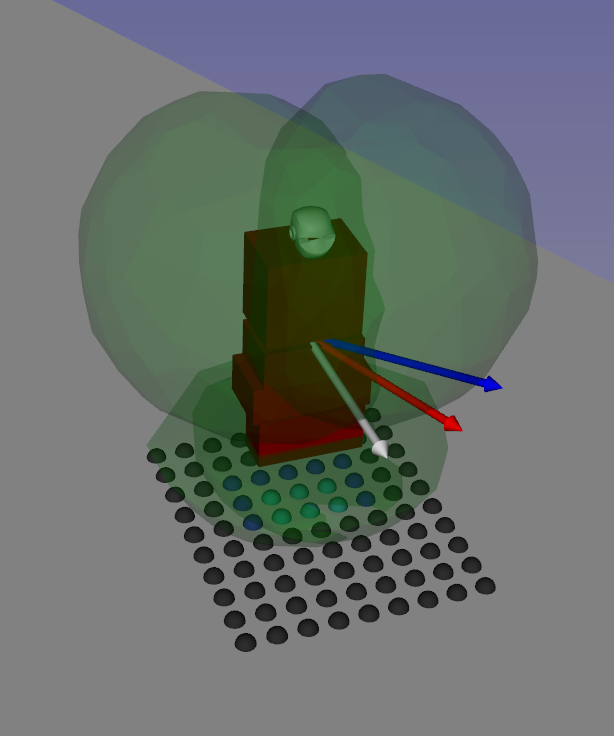
\includegraphics[width=0.42\textwidth]{Figures/Chapter_LEAS/leas_states.png}
    \caption{Robot states: (blue arrow) velocity of the robot, (white arrow) orientation, (red arrow) desired velocity and orientation, (dots) height map relative to the root configuration.}
    \label{fig:LEAS_states}
\end{figure}

The robot configuration can be seen in figure \ref{fig:LEAS_states}, from which we can get the observable states driving the actions of LEAS. The desired velocity and orientation are represented by the same vector and expressed implicitly in our states.

The observable state is a set: 
\begin{equation}
s=\{v_{o}, o_{target}, h_{o}\}
\end{equation}
with $v_{0}$ the velocity of the robot relative to its orientation, $o_{target}$ the angle between its actual and desired orientations (yaw), and $h_{o}$ a local height map of the terrain relative to its root configuration.

\begin{figure}[t]
    \captionsetup[subfigure]{justification=centering}
    %\centering
    \begin{subfigure}[t]{.49\linewidth}
    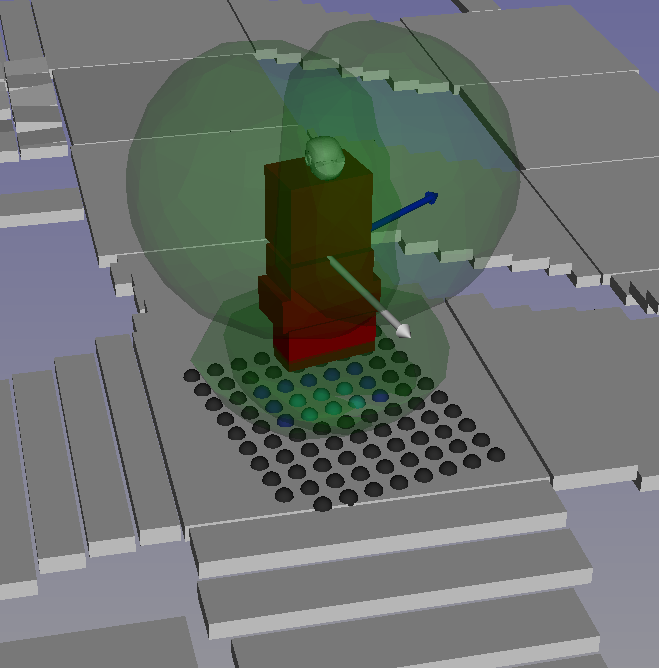
\includegraphics[width=\textwidth]{Figures/Chapter_LEAS/hm_small_vision.png}
    \caption{\label{fig:vision_hm_size_short}}
    \end{subfigure}
    \begin{subfigure}[t]{.49\linewidth}
    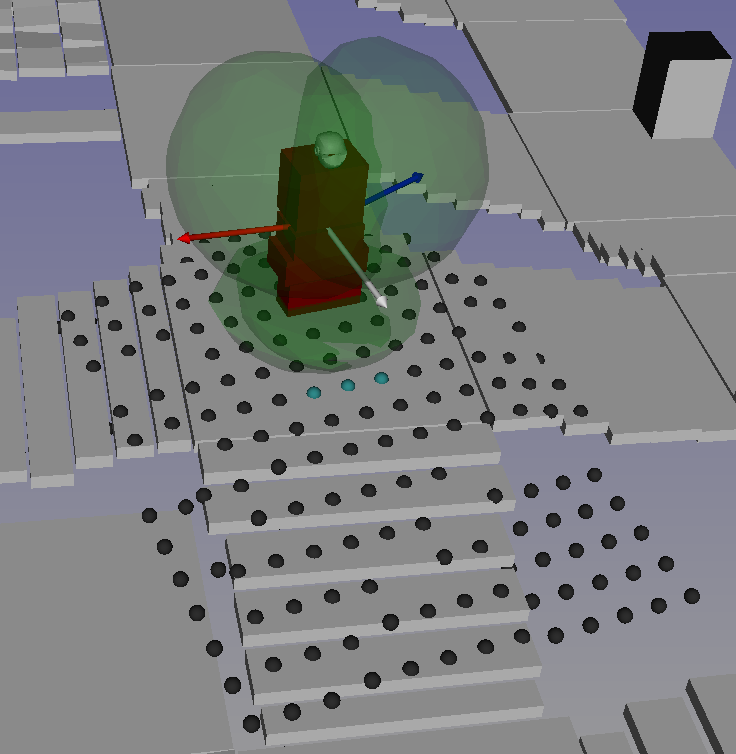
\includegraphics[width=\textwidth]{Figures/Chapter_LEAS/hm_big_vision.png}
    \caption{\label{fig:vision_hm_size_big}}
    \end{subfigure}
    \caption{Vision field of LEAS for different local height map sizes.}
    \label{fig:vision_hm_size}
\end{figure}

% - height map for the agent to understand locally its surrounding. 
% Explain the dimensions, the number of dots, the space between them. 
The dimensions of the height map are 7 values in front of the robot, 3 in the back, and 7 values on each side with a discretization step (rounded) of $15$ cm, $17$ cm, and $9$ cm respectively. This roughly corresponds to a short vision range of $110$ cm in the front, $50$ cm in the back, and $60$ cm on each side of the robot (figure \ref{fig:vision_hm_size_short}).

% Why not bigger ?
The observable height map is small on purpose as we desire a steering method with the behavior (D), to navigate locally. Increasing its visual field leads to an over-fitting on our training terrain and the emergence of path planning behavior.
Indeed, if we give too much information about the surrounding terrain (figure \ref{fig:vision_hm_size_big}), one could memorize its topography, guess its global position on it and plan its path through it, as done in \cite{rl_navigation_video_game_2020}.
Empirically, we found that $110$ cm in front and $60$ cm on each side of the robot was enough for LEAS to detect the obstacles and react in consequence.
% Is this discretization enough ?
The height map resolution of LEAS is $15$ cm, compared to previous works as \cite{RLOC, deepGait, deepLoco} that have a resolution of 2cm, 4cm, and 34cm respectively, and is sufficient to navigate the training ground and to generalize to unknown terrains. 
Increasing its resolution did not improve the learning or navigation skill of LEAS for our test scenarios, but may be required in the future for more complex scenes with elements of smaller surfaces (handrails detection for example).

\begin{figure}
    \captionsetup[subfigure]{justification=centering}
    %\centering
    \begin{subfigure}[t]{.49\linewidth}
    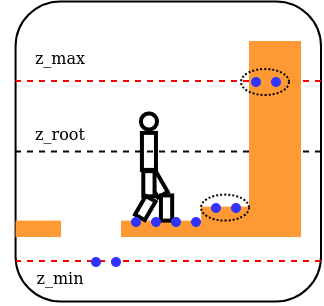
\includegraphics[width=\textwidth]{Figures/Chapter_LEAS/hm_bounded_high.png}
    \caption{Wide height map bounds}
    \end{subfigure}
    \begin{subfigure}[t]{.49\linewidth}
    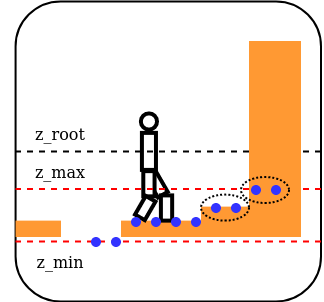
\includegraphics[width=\textwidth]{Figures/Chapter_LEAS/hm_bounded_low.png}
    \caption{Small height map bounds}
    \end{subfigure}
    \caption{Observable height map with $z_{min}$ and  $z_{max}$ relative to $z_{root}$ and (blue dot) the bounded height map values. If these bounds are (a) too large, the agent can easily detect the distant obstacle but may not dissociate the ground and the stair in front of him, or (b) too tight, the agent can better detect it but mistake the obstacle as a second stair.}
    \label{fig:height map_bounds}
\end{figure}

% What are the bounds for this relative height map ? Why not bigger bounds ?
All $z$ values in the local height map are bounded between $[z_{min}, z_{max}]$. 
The tuning of these bounds depends on the topography of the terrain where LEAS will navigate. 
Indeed, a wider interval means that the RL agents will better dissociate higher height variations (stairs and obstacles) at the cost of a lower resolution for small variations (rubbles and small slopes).
This is illustrated in figure \ref{fig:height map_bounds} where wider bounds (a) are a better representation for obstacle detection, and smaller bounds (b) make the agent more sensitive to small height variations but may mistake the distant obstacle as a stair. 
Empirically, we find a right balance $z_{max}= -0.2$ and $z_{min}= -1.4$ meters from the robot root (usually located at 1 meter from the ground), to be sufficient for LEAS to visualize both small and high variations during a pure navigation task.

\subsection{Actions\label{subsubsec:actions}}
At each step, the RL agent takes action in the environment based on the observed state. 
Our policy returns a set of actions: 
\begin{equation}
a = \{ a_x, a_y, a_z, \omega \}
\end{equation}
with $a_x, a_y, a_z$ the accelerations of the robot on each axis, and $\omega$ the angular velocity of the robot on the yaw axis. At each step $i$, the robot position q$_{pos}$, velocity q$_{vel}$ and orientation q$_{ori}$ are modified in the following order:
\begin{equation}
\begin{cases}
(a) \; q_{pos}^i = q_{pos}^{i-1} + q_{vel}^{i-1} * T \\

(b) \; q_{vel}^i = q_{vel}^{i-1} + [a_x, a_y, a_z] * T \\

(c) \; q_{ori}^i = q_{ori}^{i-1} + \omega * T 
\end{cases}
\end{equation}
with $T$, a user-defined timestep, q$_{pos}$, q$_{vel}$, and q$_{ori}$ the global position, velocity, and orientation of the robot respectively.

The velocity $q_{vel}$ and timestep $T$ impact the number of configurations along the guide path. For a constant velocity along the guide of $0.10$ m/s and $T=0.2$ seconds, the discretization step between each configuration is $2$ cm. 
We can further bound q$_{vel}$ in order to keep its norm $|\mbox{q}_{vel}| \leq v_{max}$ with $v_{max}=0.2$ m/s. %All parameters can be seen in Table \ref{tab:param}.

The choice of $T$ depends on the contact planner used. 
Empirically, we know that the contact planner \cite{AcyclicCP} has a higher success rate for discretization steps inferior to $15$ cm.
For LEAS, we choose to set $T=0.2$ seconds which results for $v_{max}=0.2$ m/s in a maximum discretization step of $4$ cm.
In the next chapters, we will further prune configurations along the guide to modify this maximum discretization step when required.
These parameters have been empirically selected to achieve the specified navigation behaviors, while computing enough configurations along the guide to be feasible by our contact planners (discussed in the next chapters).

% Why this order for the control in acceleration ? It induces a delay in the action
The order in which the robot states are updated induces a delay in the action of the agent. 
The position of the robot is updated with the previous velocity (1), then the acceleration actions update the velocity (2). As a result, the agent can observe its action impacts directly on the velocity, but not on the robot position and so its observable local height map.
%In RL, problems where the actions are not instantly applied to the states or captured by the observations have been termed as Delayed MDPs \cite{RL_delayed}. 
%Our control does not fall directly into this category as the agent can see its actions directly on the velocity. 
One can ask if inverting the order of (1) and (2), hence removing this delay on the position could improve the learning and results of our agent. 
In practice with recent RL algorithms, fixed delays of one or two steps do not matter \cite{RL_delayed_explanation} as long as the agent has enough steps left to react to an event. We verify it in figure \ref{fig:control_LEAS_learning_curves} that shows no difference in the learning of both controls with our parameters.

% Controls: why control in acceleration ?
We choose an acceleration control for LEAS, where velocity changes along the trajectory are limited by $a_{max}$, the maximum acceleration.
In our experiments, we find that small accelerations with a small timestep $T$ help the exploration and lead to a more stable training overall, as the actions have a lower impact on the system compared to a velocity control.
That is why we set a sufficiently high maximum acceleration $a_{max}=0.08$ m/s$^2$ to react to new observations, as the detection of an obstacle, but low enough to help its learning and generate smooth trajectories.

% Why not just giving the configs for each step ?
Another option is position control, where the actions directly correspond to the next root position $q_{pos}$, or similarly velocity control with a high timestep $T$, to exactly compute one configuration per footstep along the guide.
% Removed: In our experiments, this implementation does not work well with our sample-based contact planner of chapter \ref{sec:CP-SB} that prefers guide paths with a small discretization step, but is pertinent for those of chapter \ref{sec:CP-MIP} and \ref{sec:CP-SL1M}. 
While this strategy is pertinent in the contact planning context, it is also more difficult to train as it requires a few numbers but critical actions to generate a guide path.
In our experiment, training LEAS with such position control is inefficient as it drastically lowers the probability to end in a feasible state, hence requiring additional strategies to guide the exploration.
As a consequence, we prefer an acceleration control leading to stable learning of our navigation task. 
%However, this approach also implies additional implementation choices relative to the contact planners that will be discussed in the next chapters.

\subsection{Rewards}
% What do we want our robot to do ?
As written in the specifications (section \ref{subsubsec:specifications}), the behaviors we have yet to obtain are: (A) move the robot in the goal direction at the desired velocity, (C) stop if it can not go further, (E) orientate its root in the goal direction. 
We design three rewards to get these behaviors:
\begin{enumerate}
  \item[(E)] $R_{ori} = -( 1 -  \overrightarrow{q_{ori}} \cdot \overrightarrow{u}_{target} )$ \\
  with $\overrightarrow{q_{ori}}$ the unit vector representing the root orientation and $\overrightarrow{u}_{target}$ the goal direction.
  \item[(A)] $R_{dir} = -( ||\overrightarrow{q_{vel}} - \overrightarrow{v*} ||/(2v_{max}) )^2$\\
  with $\overrightarrow{q_{vel}}$ the root velocity vector, $\overrightarrow{v*}=\overrightarrow{u}_{target} \times v_{desired}$ the desired velocity vector and $v_{max}$ the max velocity norm.
  \item[(C)] $R_{alive} = 1$ 
    %$
    %\begin{cases}
    %  1, & \text{if the actual state is valid} \\
    %  0, & \text{otherwise}
    %\end{cases}
    %$
\end{enumerate}
The reward $R_{ori}$ penalizes the agent for not being oriented toward the goal (E) and $R_{dir}$ penalizes it for not moving in the desired direction at $v_{desired}$ (A). 
As both rewards are negative, using only these two encourages the agent to terminate the episode as soon as possible to avoid accumulating negative rewards. 
Therefore, we introduce another positive constant reward $R_{alive}$ that the agent gets at each step to encourage him to keep a valid configuration and continue the episode.
As a result, the agent learns that to maximize the future rewards, if it is not possible to move in the desired direction, it is better to keep the robot idle rather than terminate the episode, thus fulfilling the behavior (C).

To further smooth the trajectory, we add two rewards to punish the agent for taking large actions:
\begin{enumerate}
    \item $R_{\omega} = - | \omega / \omega_{max} |^2 $ \\
    with $\omega$ the action on orientation and $\omega_{max}$ the maximum angular velocity.
    \item $R_{acc} = - (|| [a_{x},a_{y},a_{z}] || / a_{max})^2 $ \\
    with $[a_{x},a_{y},a_{z}]$ the acceleration actions and $a_{max}$ the maximum acceleration norm.
\end{enumerate}

The resulting reward is :
$R = R_{dir} w_{dir} + R_{ori} w_{ori} + R_{\omega} w_{\omega} + R_{acc} w_{acc} + R_{alive} w_{alive}$\\
with $w_{dir}$, $w_{ori}$, $w_{\omega}$, $w_{acc}$ and $w_{alive}$ some user-specified weights.

\hfill %\break

Another possible reward design is to let $R_{dir}$ be positive as done for the High-level controller of DeepLoco \cite{deepLoco}. 
For example, we can set $R_{dir}=-(||\overrightarrow{v} - \overrightarrow{v*}||/(2 v_{max}))^2 + 1$ and remove $R_{alive}$, which in that case is strictly equivalent to our formulation above with $R_{alive}=1$ and $w_{alive}=1$.
That is why for more convenience, we separate these two rewards. 
An advantage of this separation is that we can increase $w_{alive}$, relative to the other reward weights, to further force the agent to act carefully and stay away from dangerous situations like staying too close to an obstacle. 
In our experiments, keeping $w_{alive}=1$ is sufficient to get the desired behavior (C), but setting it too high as $w_{alive}=2$ can make the agent act too safely and stay idle instead of crossing difficult obstacles.

\section{Implementation Details\label{subsec:leas-implementation}}

% Problem with using HPP like that:
% - HPP is made for scenarios on small scenes with a low number of surfaces
% - HPP can run several clients, but main use: perform scenario, close it, then restart it. No easy reset.
% - Very slow to load big scenes
% - No tool to get the height map
% - The scenes are fixed and we can not change it => One instance = one scene
% - Functions of HPP are done in C++ (fast), but may be slower if intensively called again and again as configuration validity => Need a better way to check validity (collision+reachability) => Approximations using HM.

We train LEAS using HPP software \cite{HPP} to load the terrain and the Talos robot model \cite{talos_robot}. 
To speed up the training process and learn a policy with good generalization capabilities, it is desirable to have several agents in parallel during the training to generate trajectories on one or several diverse scenes.
% Limit of HPP
While it is possible to have several clients of HPP on the same machine, this software was mainly implemented for short scenarios on small terrains, but not for intensive usage as we do in RL or to load scenes with thousands of surfaces. 

To that end, we implemented a python library to extract a height map from the scene meshes, and we present two main tools to be implemented in HPP later on: an approximation of the collision and reachability constraints using the height map, and a random terrain generator. 
Finally, we present an asynchronous version of the RL algorithm Proximal Policy Optimization (PPO) \cite{PPO_2017} that will be used in the next chapters to externally compute the contact planning sequence with a master-workers architecture.

\subsection{Validity Approximation\label{subsub:validity_approximation}}
% Explain how it is done in HPP
% Why the need to approximate it => Remove dependencies with HPP that was made for smaller scenes + Faster and simplified, enough for LeaS.
% I approximated the ROM => bounds for each point on the rel HM. Easier to tune it, without needing to cut the ROM files.
% Reachability: If all points of ROM on rel HM bellow bounds => unreachable.
% Stricter reachability: points of ROM (middle) must be above bounds.
% Collision: If one above on mid point of rel HM above bounds => collision.
The validity of a configuration is subject to two constraints: reachability $\mathcal{R}$ and collision $\mathcal{C}$.
Efficient functions are available in HPP to verify these constraints by checking if an intersection exists between either the range of motion of the robot legs or the volume representing its trunk, and the terrain surfaces. 
However, in our first version of LEAS \cite{LEAS}, the computation time of these validation functions was significant (more than 15\% of the computation time), and as a consequence, we opted for a faster and more flexible implementation of these constraints.

\begin{figure}[ht]
    \captionsetup[subfigure]{justification=centering}
    \centering
    \begin{subfigure}[t]{.35\linewidth}
    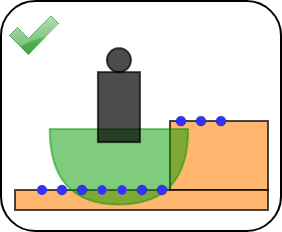
\includegraphics[width=\textwidth, height=4cm]{Figures/Chapter_LEAS/approx0.png}
    \caption{\label{fig:approximation_validity_0}}
    \end{subfigure}
    \begin{subfigure}[t]{.35\linewidth}
    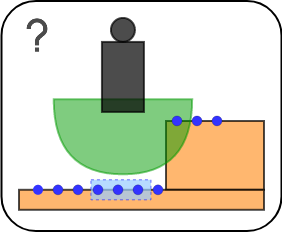
\includegraphics[width=\textwidth, height=4cm]{Figures/Chapter_LEAS/approx1.png}
    \caption{\label{fig:approximation_validity_1}}
    \end{subfigure}
    \begin{subfigure}[t]{.35\linewidth}
    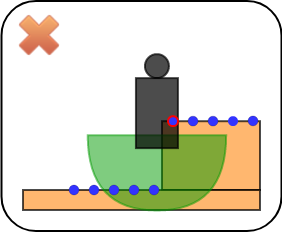
\includegraphics[width=\textwidth, height=4cm]{Figures/Chapter_LEAS/approx2.png}
    \caption{\label{fig:approximation_validity_2}}
    \end{subfigure}
    \begin{subfigure}[t]{.35\linewidth}
    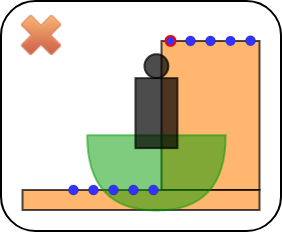
\includegraphics[width=\textwidth, height=4cm]{Figures/Chapter_LEAS/approx3.png}
    \caption{\label{fig:approximation_validity_3}}
    \end{subfigure}
    \caption{Approximated validity conditions: (Green) robot range of motion, (blue) height map. Configuration (a) is valid, (b) is valid with $\tilde{\mathcal{C}}$ and $\tilde{\mathcal{R}}$ but invalid with $\tilde{\mathcal{R}^*}$ where none of the highlighted blue dots are reachable, (c) and (d) are valid with $\tilde{\mathcal{R}^*}$ but in collision.}
    \label{fig:approximation_validity}
\end{figure}

We approximate the collision and reachability constraints by $\tilde{\mathcal{R}} \subset \mathcal{R}$ and $\tilde{\mathcal{C}} \subset \mathcal{C}$ respectively, both using the local height map $H$ relative to the robot root (Figure \ref{fig:approximation_validity}).
Offline, we assign to each point $p_i \in H$, some reachability $\tilde{\mathcal{R}_i}$ and collision $\tilde{\mathcal{C}_i}$ constraints on its height $z_i$. 
A point $p_i$ respects $\tilde{\mathcal{R}_i}$ if it lies inside the robot range of motion, and respects $\tilde{\mathcal{C}_i}$ if it lies outside and under the robot trunk volume. 
The approximated reachability condition is valid if:
\begin{equation}
    H \in \tilde{\mathcal{R}} \Rightarrow \exists p_i \in H, p_i \in \tilde{\mathcal{R}_i}
\end{equation}
The approximated collision condition is valid if:
\begin{equation}
    H \in \tilde{\mathcal{C}} \Rightarrow \forall p_i \in H, p_i \in \tilde{\mathcal{C}_i}
\end{equation}
These approximations require the robot root to only rotate on the yaw axis when navigating, that is a common assumption for biped locomotion \cite{deits2014FootPlanMI}.

One drawback of using a single-layer height map for this validity condition is its limitation to environments without an upper floor or ceiling.
% Collision detection
Regarding $\tilde{\mathcal{C}}$ constraint, the trivial case is that if a point $p_i$ lies inside this volume, there is a collision (figure \ref{fig:approximation_validity_2}). However, we do not know if there is a collision if a $p_i$ lies right above the robot. 
There are two cases: first, the robot is under an object (ceiling) and not in collision; second, the robot is inside the object (e.g. wall) and so is in collision (figure \ref{fig:approximation_validity_3}).
From the height map, we cannot distinguish these cases and thus we choose to consider both as a collision.
% Conclusion of this drawback
As all our test terrains do not contain an upper floor and we do not perform any locomotion task like passing under a gate, such an approximation is sufficient. 
In the future, another solution will be required to navigate such scenes like using a two-layers height map or voxels to better approximate the terrain geometry or using alternative validity conditions.

% No longer true with the formulation above
% is that it considers upper floors and ceilings as obstacles. However as we do not perform scenarios as passing under a gate or crouching to move under a low ceiling, such approximation is acceptable. A solution to this limitation in a future work could be to use two height maps, one for the closest ground floor and a second one for the upper ceiling.  \stn{ou simplement pas mettre le pied plus haut que le torse ?}

% Depending on the discretization of the height map, it can happen that the reachability constraint is not fulfilled even if graphically, we can see that the ground is reachable. 
% If a config is invalid with the approx, recheck :
% (1st option) Use isConfigValid of HPP.
% (2nd option) Create a convex hull from the approximated reachability bounds, and check if there is an intersection with any of the potential surfaces
Another limitation comes from the height map resolution that can fail to approximate the constraints $\mathcal{R}$ and $\mathcal{C}$.
% What happens
% Reachability
On reachability, a low height map resolution can fail to visualize a scene composed of small and spaced surfaces. Consequently, it can wrongly consider that $H \notin \tilde{\mathcal{R}}$ (i.e. the terrain under the robot is not reachable) when in reality $H \in \mathcal{R}$.
To remove such cases, we can reconfirm the invalidity of the configuration with the full constraint $\mathcal{R}$, resulting in a reasonable trade-off between computation time and completeness.
% Collision
As for the collisions, the opposite can happen where a collision is not detected by the approximation, $H \in \tilde{\mathcal{C}}$, when in reality $H \notin \mathcal{C}$. Consequently, only the full validation $\mathcal{C}$ can detect these cases.
In practice, our steering method learns to keep a safe margin between the obstacles and the robot trunk to avoid collisions and so, implicitly avoid these collision detection failures. 
Therefore, we choose to rely on the approximated constraint $\tilde{\mathcal{C}}$ that is sufficient to detect most of our robot trunk collisions.
% Trade-off
%In our implementation, we opt for a trade-off between the fast to compute approximated validity constraints $\tilde{\mathcal{R}}$ and $\tilde{\mathcal{C}}$ checked at every step of the guide path generation, where the full reachability condition $\tilde{\mathcal{R}}$ is only performed to confirm the invalidity of a root configuration.
\begin{figure}[ht]
    \centering
    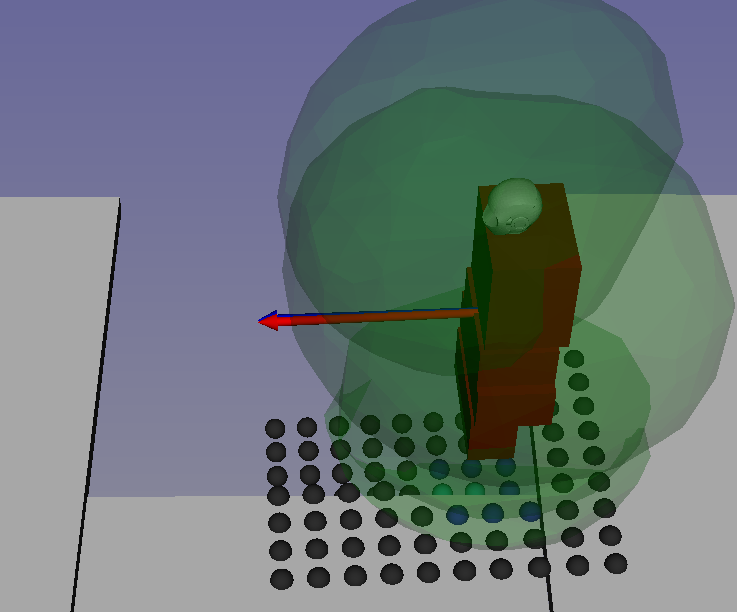
\includegraphics[width=0.42\textwidth,height=4.5cm]{Figures/Chapter_LEAS/hole_scenario_above_void_p1.png}
    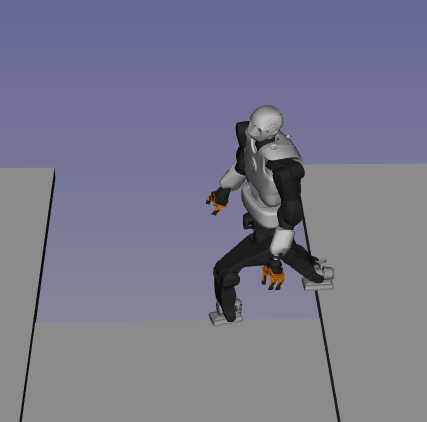
\includegraphics[width=0.42\textwidth,height=4.5cm]{Figures/Chapter_LEAS/hole_scenario_above_void.png}
    \caption{Valid configuration with $\tilde{\mathcal{C}}$ and $\tilde{\mathcal{R}}$ leading to a blocking configuration above the hole.}
    \label{fig:hole_scenario_above_void}
\end{figure}

Finally, we add one additional constraint to further improve the guide quality for the biped locomotion task. 
One default of the original validity function is that configurations above the void but touching the edge of the terrain with the range of motion are considered valid (Figure \ref{fig:hole_scenario_above_void}), leading to infeasible trajectories by our contact planners.
To avoid these configurations, we add another validity condition on the height map $H^*$ located directly under the root of the robot to be reachable at all times (dots under the robot in Figure \ref{fig:approximation_validity_1}). 
We name the reachability constraint with the stricter condition $\tilde{\mathcal{R}^*}$ where:
\begin{equation}
    H \in \tilde{\mathcal{R}^*} \Rightarrow \exists p_i \in H^*, p_i \in \tilde{\mathcal{R}_i}
\end{equation}
With this strategy, configurations are considered invalid if the robot stands above the void. 
It can be limited on terrains with very spaced surfaces, but in all our scenarios this condition offers good results in terms of guide path quality.
This solution was not yet implemented in our first version of LEAS \cite{LEAS} where we learned by reinforcement such additional constraints using the contact planner as a guide path validator, hence leading to longer training.
%This leads to the generation of a guide path with fewer states above the void and so a faster computation time with our contact planners.

In the context of RL, where the agents perform millions of steps, the approximations $\tilde{\mathcal{R}^*}$ and $\tilde{\mathcal{C}}$ significantly improve the training time.
While the gains in computation can not be fairly compared due to their difference in programming language and optimization, our implementation resulted in an average of 20 times faster computation time compared to the full constraints $\mathcal{R}$ and $\mathcal{C}$, hence enabling us to train and test more models.

\subsection{Terrain Generator\label{subsub:terrain_generator}}

\begin{figure}[ht]
    \centering
    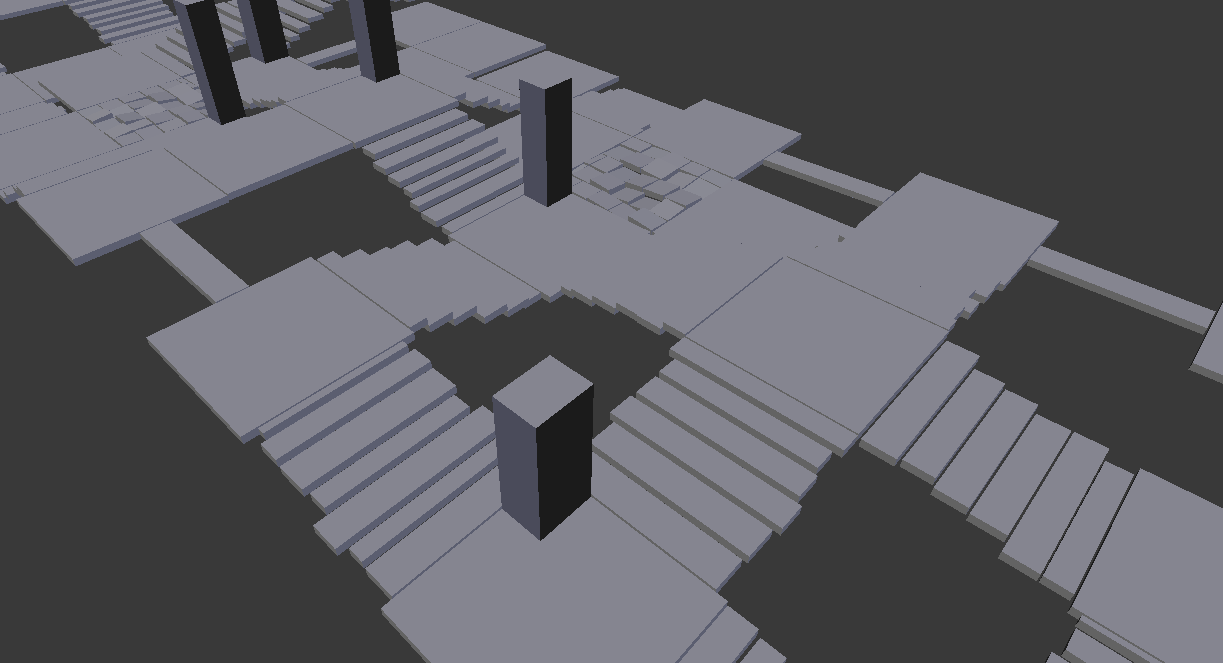
\includegraphics[width=0.7\textwidth]{Figures/Chapter_LEAS/random_scene_tiles_example.png}
    \caption{Example of a random scene generated, containing different types of tiles connected. Initial tiles: flat ground with and without obstacles. Transition tiles: rubbles, bridge, and stairs.}
    \label{fig:random_scene_gene_tiles_example}
\end{figure}

% Originally made by daeun, and adapted by me to produce arenas of size NxM
% That is somehow a huge part of my work that was needed for LeaS.
% Give a link to the code as well, but say that some fix need to be made.
Our goal is to train one policy to navigate through all our test scenarios.
To improve its generalization capability, our RL agent has to learn on various terrains. 
To that end, we extended the library used in \cite{sl1m_v2} to generate random terrains composed of rubbles, stairs, bridges, and obstacles. The code is available on GitHub \cite{random_scene_gen}.

This library generates a terrain that we can divide into tiles. 
Each tile belong to two categories: \textit{Initial} or \textit{Transition} (figure \ref{fig:random_scene_gene_tiles_example}). 
The first category \textit{Initial} contains two types of tiles: flat ground with or without obstacles. 
The second category \textit{Transition} connects two \textit{Initial} tiles and contains three types: rubbles, bridge and stairs.

We represent the terrain as a grid where each cell is a fixed-sized tile. Starting from an \textit{Initial} tile, we build a tree filling pseudo-randomly its empty neighbors. Each \textit{Transition} is unique as the characteristics of each surface composing it are random, but also depend on the height of the tiles it connects.

At the end of the terrain generation, we can identify all the links created. 
A link is defined as a sequence of \textit{Initial} - \textit{Transition} - \textit{Initial} tiles in a line, and that we can further divide into several categories in function of their difficulty. 
Finally, we extract the possible starting positions for the robot on each link, corresponding to areas on the \textit{Initial} tiles. 

Terrains generated by this library can contain enough elements, depending on the grid dimension and the random seed, for the agent to develop its navigation skill, then generalize to our test scenes that contain the same type of transitions.



% Some limitations of using this library to generate terrains for the training
% (1) All tiles have the same size, it can be a problem depending on the observable height map of the agent, for example, it will never learn how to climb very long stairs if the hm is too big.
% (2) It is limited to the kind of transitions that are implemented. Very different obstacles as walking on plateforms or weird scenarios may not work with an agent trained on our terrain. Even though our arena is big and contains enough element for the agent to figure out most of our test scenarios.
% (3) These scenes are still fixed, no dynamic elements. Ok for our test scenarios.
% (4) The quality of the agent depends on the scene it's been trained on. We have to carefully see if the generated scene contain enough of each tile types.
Some limitations come with the use of this library for our training.
The first is that all the tiles have the same dimensions, fixed to 2x2 meters for all our training scenes. 
Its dimensions have to be carefully tuned according to the size of the observable height map by the agent.
Indeed, a too large visual field could lead the agent to specialize in navigating scenes with this specific tile size, e.g. the agents can specialize in crossing stairs or bridges of 2 meters. 
In our experiments, with a visual field of $110$ cm in the front (Section \ref{subsubsec:states}), learning on a terrain of 2x2 meters tiles is sufficient to learn local navigation behaviors.
The second limitation is that even though the \textit{Transition} and obstacle tiles are unique and randomized, they still fall into the same categories (i.e. stairs, rubbles, bridge, obstacle). Consequently, we could question the ability of the agent to navigate on very different terrains. Empirically, this was not a problem to generalize to all our test scenarios mostly containing the same type of elements, however, a higher diversity may be required in the future.
The performance of the agent also depends on the size of the terrain it has been trained on. We had to generate several random arenas before finding one having enough elements and links. 
In our experiments, terrains of dimension 5x30 are the maximum we can have in HPP as the terrain loading and processing times exponentially increase with the number of surfaces.

% Options tried
% (1) All parallel agents during the training evolves on different terrain, possibility to change this terrain, going from an easy one first to a more difficult one later on => Curriculum learning. Then we run one or several contact planners for each type of terrain, that will compute the CP only for these terrains.
% (2) Have just one huge scene that has enough diversity of obstacles / transitions to learn how to generalize.
% A combination of (1) and (2) is also possible.
 Finally, several options can be explored to learn from the random scenes generated.
 We can have several parallel agents learning in different scenes or modifying the scene during the training.
 We can also use the difficulties of each link in the scene to perform curriculum learning \cite{curriculum_learning_survey}, starting from the easiest link to the most difficult one.
 In a previous test, we ran several agents during the training on different terrains and following such a curriculum learning, for example starting from flat ground, then switching to stairs, and finally, a terrain randomly generated. However, it did not further improve the learning time, as our agent is already able to learn quickly from a single 5x30 random scene without these methods.
 
 
\subsection{Master-Workers Architecture: Asynchronous contact planners\label{subsub:leas:master_worker}}

% Why did I pick PPO (online) and not an offline RL algo
Several state-of-the-art RL algorithms are available and can be separated into different groups, each presenting some pros and cons, and that can lead to various results depending on their hyperparameter tuning and the task to perform \cite{RL_that_matters, RL_that_matters_OnPolicy}. As a consequence, it can be difficult to judge which algorithm to use for a given task other than empirically. 
%However, some comparisons are available to guide our choice \cite{compare_PPO_TD3_SAC_DDPG}.
Among the most recent and popular RL algorithms, we have Proximal Policy Optimization (PPO) \cite{PPO_2017} in the category of on-policy algorithms, and Twin Delayed DDPG (TD3) \cite{TD3_2018} and Soft Actor-Critic \cite{SAC_2018} in off-policy.
% What do we try ?

In this work, we experimented on PPO and TD3, both implemented in Stable Baseline \cite{stable-baselines} that we can easily adapt for our task.
% What are the main pros and cons
Off-policy algorithms, such as TD3 and SAC, are known to be more sample efficient but can lack stability compare to on-policy RL algorithms.
% What do we pick in the end ?
% Note: TD3 is hard to tune, it did not converge after 3M steps, when PPO already converged.}
That is why many recent works in RL use PPO \cite{survey_rl_animation_pettre_2022} that, to this day, can be easier to tune and more stable during the learning, even for tasks that require data-efficiency as \cite{openai2019dota}.
%The learning of LEAS without a contact planner, which is a pure navigation task can be learned efficiently with PPO as in \cite{compare_PPO_TD3_SAC_DDPG} for a boat navigation task.
In our first version of LEAS \cite{LEAS}, the training with PPO was slow due to its poor sample efficiency (order of hours without contact planning and tens of hours with our sample-based contact planner). %At that time, using off-policy RL algorithms was a more pertinent choice.
However, this issue was fixed with the optimizations and approximations discussed in the previous section thus making both off- and on-policy pertinent choices.
We tested TD3 and PPO for our navigation task and we observed with TD3 a slower and less stable convergence than PPO, using the default hyperparameters as defined in Stable Baseline or with manual tuning.
As a result, we decided to use PPO to learn LEAS.

% What is the main problem of LEAS design, how to modify PPO to make it works ?
% Why only asynchronous for the CP ? Why master-worker ? Are there some limitations / alternatives ? => Limitation of our software + exchange of datas between processes + the CP is the only long thing to compute and just need the guide path to be done.
Given the design of LEAS, we have two components to consider during the training. First, our steering method is a policy taking actions in the environment and saving the state sequence as a guide path. Second, the contact planner computes the contact sequence along it and gives feedback on its result to LEAS.
%We do not define the feedback in this section that depends on the contact planner used and the type of reward we want to implement.
In this design, the main limitation comes from the contact planning validation at the end of each episode. 
If we simply perform this contact planning inside each agent, as all parallel agents are steps synchronous (or trajectory synchronous), if one agent computes a contact sequence, all the others have to wait for it to finish. Consequently, the computation time increases with the number of agents in parallel.
We have two solutions to solve this problem: (a) Compute all trajectories asynchronously or (b) compute all guide paths synchronously and perform P2 asynchronously.
We implemented both solutions (a) and (b) using a master-worker architecture (Figure \ref{fig:architecture_master_worker}).
\begin{figure}[t]
    \captionsetup[subfigure]{justification=centering}
    %\centering
    \begin{subfigure}[t]{0.9\linewidth}
    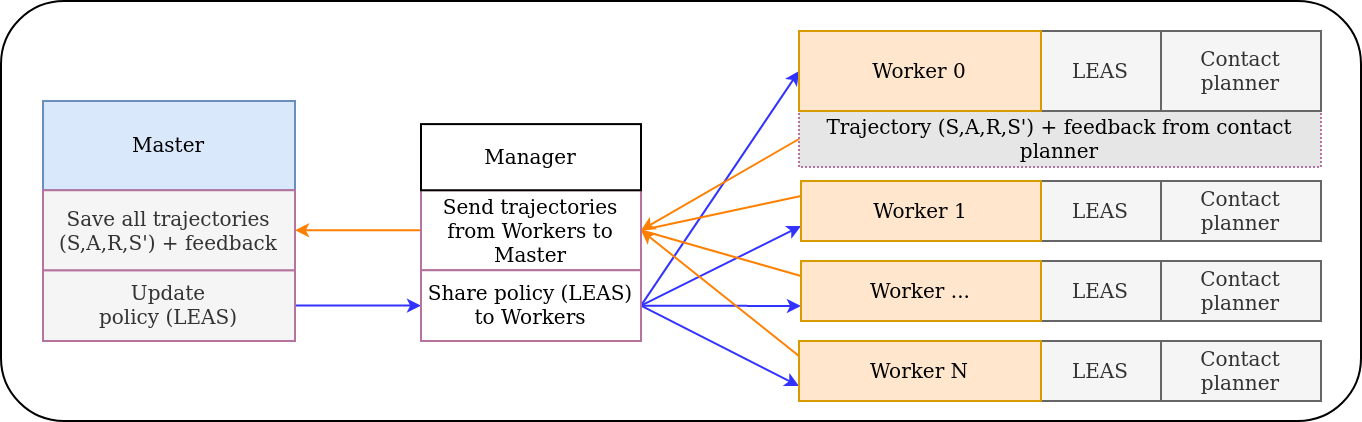
\includegraphics[width=\textwidth]{Figures/Chapter_LEAS/architecture_master_worker_0.png}
    \caption{Asynchronous guide path and contact planning}
    \label{fig:architecture_master_worker_synchronous}
    \end{subfigure}
    \begin{subfigure}[t]{0.9\linewidth}
    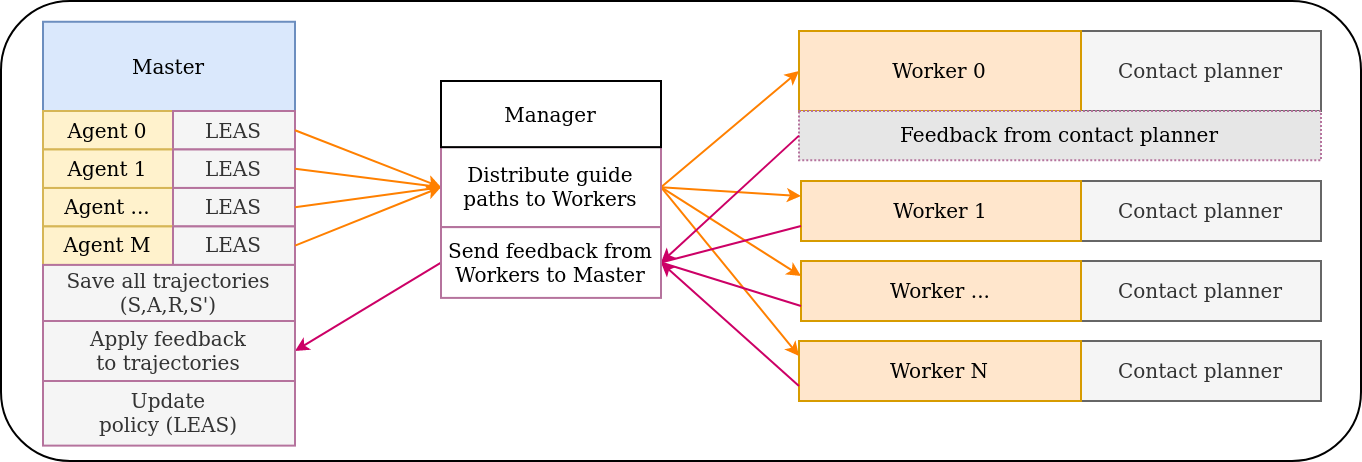
\includegraphics[width=\textwidth]{Figures/Chapter_LEAS/architecture_master_worker_1.png}
    \caption{Synchronous guide path and Asynchronous contact planning}
    \label{fig:architecture_master_worker_asynchronous}
    \end{subfigure}
    \caption{Two versions of Master-Workers architecture to learn LEAS plugged to a contact planner.}
    \label{fig:architecture_master_worker}
\end{figure}

% Solution A : all asynchronous
Solution (a) dissociates the learning operated by the master and the trajectory generation performed by the workers (so-called distributed RL).
The advantages of this method are its scalability, as we can add during the learning as many agents as desired that can run on different machines, and its modularity as the agents can be initialized on new terrain and stopped if needed.
This method is used in IMPALA \cite{impala2018} running 32 CPUs and RAPID \cite{openai2019dota} with 500 CPUs, showing impressive results to learn challenging and complex tasks.
However, this method also requires a lot of data exchanges between the RL algorithm and the workers as explained in \cite{evol_vs_rl_majid_2021}. 
The load on the network increases with the number of data (the trajectories) exchanged between the master and the workers, plus the parameters (policy network) that must be shared with all the workers after each update.
As a consequence, this approach can result in some hardware and implementation limitations depending on the available resources, and a possible delay in the policy of the asynchronous agents.

% Solution B : Guide path synchronous and contact planning asynchronous
The other solution (b) lets the master generate all the trajectories with one or several synchronous agents, then dispatch the guide paths generated to the workers that compute P2 and return the result to the master.
It is a solution specifically adapted to our problem and simple to implement that can be added on top of any on-policy or off-policy RL algorithm. 
%One or several agents generate synchronously some guide paths, that are shared with external workers that compute the contact sequence. Then, they return their feedback to the master for learning. 
The key advantage of this method is the reduction of data exchanges between the master and the workers. Only the guide path, a sequence of positions and orientations, and the feedback from the contact planner transit on the network.
However, if the guide path generation P1 is faster than P2, we can observe some lags between the synchronous agents and the workers. That is why we need to balance their number or add more workers to follow the flow. Also, the parallel agents during the learning run on environments that can not be changed manually, making it a simple but less modular method overall compared to (a).

In our experiments, solution (a) led to a bottleneck on our hardware due to the amount of data exchanged, and going for pre-made implementation as IMPALA was not necessary for our problem that only requires a few hours of training compared to the tasks solved in \cite{impala2018, openai2019dota}.
Therefore, we opted for solution (b) which is a good compromise between synchronous and asynchronous steps.
In the future, we would like to take a look at fully decentralized architectures \cite{DD_PPO} that solve the problem of network overload by sharing only the gradients for training.

With setup (b), we will now perform several tests on basic scenarios with LEAS without contact using the original PPO algorithm, then plug it into a contact planner using our modified PPO version to analyze its impact on the trained policy.

% Say that for the results bellow, we do not use the contact planners, equivalent to a contact planner that returns that all trajectories are succesful and returns last index of obs.

\section{Results\label{subsec:leas-results}}

\begin{figure}
    \centering
    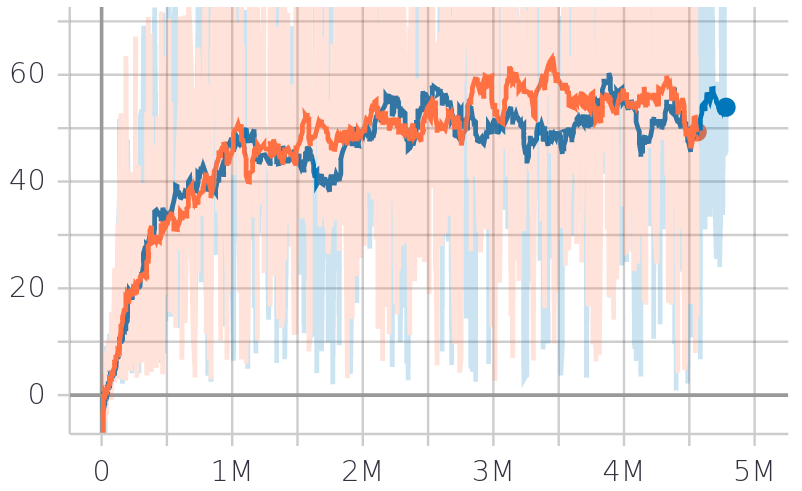
\includegraphics[width=0.6\textwidth]{Figures/Chapter_LEAS/learning_curves_P1.png}
    %\begin{subfigure}[t]{0.49\linewidth}
    %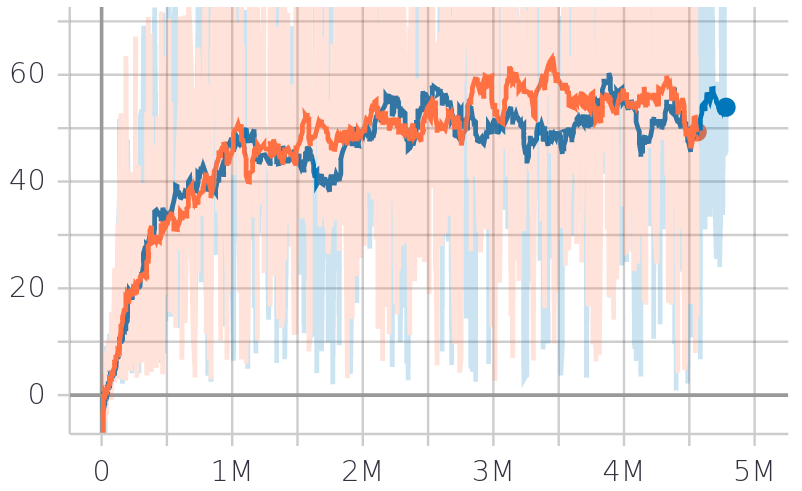
\includegraphics[width=\textwidth]{Figures/Chapter_LEAS/learning_curves_P1.png}
    %\caption{}
    %\end{subfigure}
    %\begin{subfigure}[t]{0.49\linewidth}
    %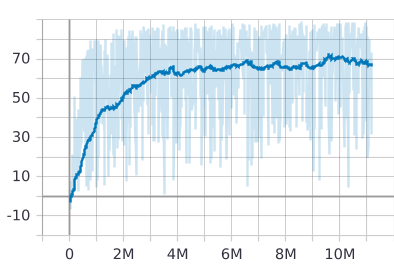
\includegraphics[width=\textwidth]{Figures/Chapter_LEAS/learning_curve_leas_p1.png}
    %\caption{}
    %\end{subfigure}
    \caption{Learning curves of LEAS without contact planner feedback (pure navigation task) with an acceleration control (Orange) with delay, (Blue) without delay on the position update.}
    \label{fig:control_LEAS_learning_curves}
\end{figure}

\begin{table}[tb]
\begin{center}
\caption{Parameters}
\begin{tabular}{|c|c| c |c|c|}
 State & $81$ && Max Episode Length & $800$\\
 Actions & $4$ && Parallel agents & $6$\\
 $a_{max}$ & $0.08$ m/s$^2$ && Workers & $0$ \: or \: $6+$ \\
 $v_{max}$ & $0.2$ m/s && Batch size & $4096*M$\\
 $v_{desired}$ & $0.1$ m/s && Mini-Batch size & $256$\\
 $\omega_{max}$ & $\pi/9$ rad/s && Learning rate & $[5e-4,1e-5]$\\
 Timestep $T$ & $0.2$ s && Noptepochs & $10$\\
 Local height map $H$ & 10x14 && Discount Factor ($\gamma$) & $0.97$\\
 $z_{max}$ & $-0.2$ m  && Clip range & $0.2$\\
 $z_{min}$ & $-1.4$ m &&
 $w_{ori}$ & $0.4$ \\
 $w_{dir}$ & $1.0$  &&
 $w_{acc}$ & $0.1$ \\
 $w_{\omega}$ & $0.1$  &&
 $w_{alive}$ & $1.0$
\end{tabular}
\label{tab:param}
\end{center}
\end{table}

\begin{figure}
    \centering
    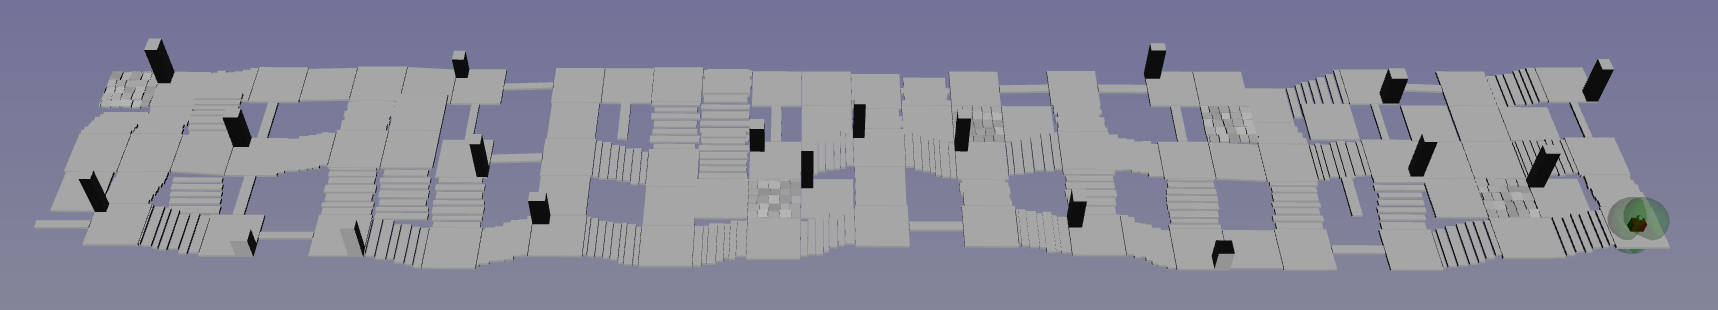
\includegraphics[width=\textwidth]{Figures/Chapter_LEAS/arena_5x30.png}
    \caption{Training ground of LEAS: a 5x30 arena (corresponding to 10x60 meters) composed of 86 links: 17 bridges, 31 stairs, 8 rubbles, and 30 flat ground with obstacles. All links are two-way and have different elements characteristics and slopes.}
    \label{fig:arena_5x30}
\end{figure}

% Explain what do we use
We use the HPP software \cite{HPP} and the humanoid robot Talos model \cite{talos_robot}. Our algorithm is implemented in python using the PPO implementation of Stable Baselines \cite{stable-baselines} modified for our Master-Workers architecture.
% Parameters
All parameters in the environment and hyperparameters to control the learning process can be seen in Table \ref{tab:param}. We use the terrain generator described in \ref{subsub:terrain_generator} to generate the 5x30 training ground in Figure \ref{fig:arena_5x30}.

% Explain parameters for the ENV
% - timestep => Why this value
We set a fixed timestep value $T =0.2$ seconds, which corresponds to a maximum distance between each state on the path of $4$ cm for $v_{max}=0.2$ m/s, and $2$ cm for $v_{desired}=0.1$ m/s.
% - number of steps max => Important to explore enough, not do only links and not be stuck somewhere.
Each episode has a maximum length of $800$ steps, meaning that the guide path can contain up to $800$ states (maximum distance of 32 meters). 
During the training, the robot has to navigate the terrain at the desired velocity while keeping a valid state ($\tilde{\mathcal{R}^*}$ and $\tilde{\mathcal{C}}$).
To further guide the learning, we initialize each episode as follows: first, the robot has to cross a link, i.e start from an initial tile and navigate through a transition tile (stairs, rubbles, or bridge), then, it has to follow a new random goal direction that is updated every $n_{rand} \in [200,800]$ steps.
The first goal prioritizes the task of crossing a link that we will perform in all our basic scenarios, while the others often lead to a dead-end or a difficult path where the agent will have to learn if it has to stop or has the ability to cross it.

% Param for learning
We linearly decay the learning rate from $5e^-4$ to $1e-5$ over 2 millions steps and set a discount factor $\gamma = 0.97$. 
A method to tune the discount factor is to calculate the half-life $\tau = \frac{1}{1-\gamma}$ which roughly corresponds to the number of steps considered to adapt the agent behavior. For LEAS, it is equal to $\tau = \frac{1}{1-0.97} \approx 33$ steps. 
As a result, steps from $[0,33]$, $[33,66]$, $[66,99]$, $[99,\infty]$ will roughly account for $63\%$, $23\%$, $8\%$ and $6\%$ of the sum of discounted rewards respectively. 
The distance traveled by the RL agent after 33 steps is equal to 66 cm and 132 cm for velocity equals to $v_{desired}$ and $v_{max}$ respectively.
% Notes: integral 0 to inf (0.97**x) = 32.8  => from 0 to 33=20.8 => from 33 to 66=7.6 => from 66 to 99 = 2.78. So most of the reward comes from 0 to 33 (64%), from 33 to 66 (23%), from 66 to 99=8%. If discount factor 0.98 : half-life at 50 => 0-50:64% => 50-100:23% => 100-150=8%
We emphasize that we want to learn a steering method to navigate locally and that the agent only needs to think about its very near future. For example the detection of an obstacle should impact its action only when close to the robot (distance inferior to 1 meter).

% Number of workers
In this chapter, the number of workers planning contacts is set to 0 as we train LEAS for a pure navigation task without a contact planner. In our experiment, the number of synchronous workers is limited to 6 due to hardware limitations.

% Explain choices for the RL parameters used:
% - size of network with PPO : 256x128x64
The PPO actor and critic are two distinct networks with hidden layers of size 128x64x32. Tuning the number of nodes and hidden layers in the machine is empirical and depend on the task to perform. In general, deeper networks with more nodes means a better capability to solve very complex tasks and less under-fitting. However, it also means more parameters to train and can be prone to over-fitting. In our experiments on LEAS, we found no noticeable difference between 2 or 3 hidden layers and nodes number ranging from 64-256. However, we increased the network size of 64x64 from the first version of LEAS \cite{LEAS} for more potential scalability in our tests in terms of observations and contact planners.

We train LEAS without a contact planner and evaluate the model after 5 million steps corresponding to around 1 hour of training on a PC with an Intel Core i7-8700 (12 cores, 3.20Ghz, 16GB ram). Learning curves can be seen on figure \ref{fig:control_LEAS_learning_curves}.

\subsection{Comparison: Steering Method Designs\label{tab:compare_sm_charac}}

\begin{table}[ht]
\caption{Comparison of the steering method characteristics.}
\begin{center}
\begin{tabular}{ |c|c|c|c| }
\hline
Steering Method & RB-Lin & RB-Kino & LEAS (ours)\\
\hline
Goal Connection & 
\thead{\textcolor{red}{Exact}\\pos,ori} & 
\thead{\textcolor{red}{Exact}\\pos,vel,acc,ori}  & 
\thead{\textcolor{blue}{Near}\\pos}
\\
\hline
Dynamic constraints &
\thead{\textcolor{red}{1}\\$v_{max}$} &
\thead{\textcolor{red}{2}\\$v_{max},a_{max}$} &
\thead{\textcolor{blue}{3}\\$v_{max},a_{max},\omega_{max}$}
\\
\hline
Terrain aware &
\thead{\textcolor{red}{No}} &
\thead{\textcolor{red}{No}} &
\thead{\textcolor{blue}{Yes}}
\\
\hline
\thead{Path planning\\dependant} &
\thead{\textcolor{red}{Yes}} &
\thead{\textcolor{red}{Yes}} &
\thead{\textcolor{blue}{No}}
\\
\hline
\end{tabular}
\end{center}
\end{table}

% Compare it to SM : RB-Kino and RB-Lin
% Show the difference between all SM :
% - RB-Kino connects exactly two points and its shape is relative to the two configs linked. 
% Advantage: connect exactly and we can control the acceleration and velocity at the goal + control on the acceleration.
% Disadvantage: Requires path planning to find the acc/vel/orientation at the arrival to obtain a valid guide path. Totally dependant on the path planning + can not be used for a control with a remote + does not consider the terrain to generate the trajectory.
% - RB-Lin connects exactly two points and do not perform DIMT, it's just a linear interpolation in velocity, orientation and position. No control on the acceleration.
% Advantage: Very simple to implement.
% Disadvantage: Also requires path planning as a line guide path is not sufficient very often to climb stairs + does not consider the terrain to generate the trajectory.
% - LEAS does not connect exactly two points and will just end up near the goal position.
% Advantage: Less dependant on path planning as the goal state is smaller (only position) and it can locally navigate depending on the terrain + control on the acceleration max.
% Disadvantage: No control on the velocity and orientation at the goal. Does not end exactly on the goal.
We compare LEAS, a flexible alternative to our previous steering methods. Their characteristics can be seen in Table \ref{tab:compare_sm_charac}.

\hfill

% Goal connection
\noindent \textbf{Goal connection}:
RB-Kino \cite{kinodynamic_sm_2017} and RB-Lin \cite{AcyclicCP} are two steering methods that connect exactly some initial and goal configurations in position, velocity, and orientation. 
% RB-Kino
RB-Kino uses the Double Integrator Minimum Time \cite{DIMT} to also add a constraint on the acceleration.
% LEAS
LEAS does not exactly connect the initial and goal configurations as it is trained to follow a given goal direction. Consequently, it can at best end up near the goal position.
The capability to connect exactly two configurations is needed in robotics for hand manipulation. Arguably, in locomotion, this accuracy is not required in most scenarios.
This is especially true on long paths with key waypoints to sequentially reach up to a distant objective, where passing close enough to each waypoint is sufficient.
As LEAS uses a target direction instead of a target configuration, it also enables us to use a joypad-like control, which is equivalent to a very distant moving target that the agent tries to reach. We simulate this kind of control for the training of LEAS by randomly repositioning its goal.

\hfill

% Dynamic constraints
\noindent \textbf{Dynamic constraints}:
% RB-Lin constraints
RB-Lin is a modified linear interpolation that is constrained in orientation and velocity. It first rotates the robot toward the target at $\omega_{max}$, then moves toward it at $v_{desired}$.
% RB-Kino constraints
RB-Kino requires two parameters $v_{max}$ and $a_{max}$ that act as strict constraints on both velocity and acceleration. However, no constraints are set on the angular velocity $\omega_{max}$ and this can be a problem as we will see in chapter \ref{sec:CP-SB}. 
%\textcolor{red}{TO CHECK, no constraint on angular velocity ? Why Pierre did not change it? He prefered starting with a higher init velocity to avoid this problem.}
% LEAS constraints
On the other hand, the control of LEAS constrains each configuration with $v_{max}$, $a_{max}$, $\omega_{max}$. 
In this thesis, we only use quasi-static contact planners, so $v_{max}$ and $a_{max}$ are considered during the guide path planning but not the contact planning phase. However, using LEAS with a kinodynamic contact planner is a possibility for future work.

\hfill

% Terrain aware + path planning
\noindent \textbf{Terrain-aware and path planning}:
RB-Kino and RB-Lin both require a path planning algorithm to place additional waypoints to reach a distant goal. In contrast, LEAS can observe its surrounding terrain and can locally navigate it in a given direction, hence removing the need for path planning on basic scenarios (i.e. crossing a link). 
In complex scenarios, path planning algorithms can also be used to place waypoints followed by LEAS. 
In this work, LEAS can navigate the same waypoints computed by the RRT with RB-Kino. In future work, having an RRT with LEAS in the same manner as RL-RRT \cite{RL_RRT} is a work in progress.

\hfill

Finally, we recall the main advantage of LEAS over our previous steering methods which is the use of Reinforcement Learning that, through the trajectory validation by the contact planner, can change its behavior to fit it and generate more likely feasible paths.

\subsection{Test Scenarios\label{subsub:leas:test_scenarios}}

As LEAS does not connect exactly with the goal position, we consider the goal as reached when the distance from the current state on the guide path to the goal is lower than a distance threshold $\epsilon$ set to $20$ cm for all our scenarios.

% Show behaviour:
% [0] Navigate while keeping a desired velocity => Show acceleration, velocity, orientation, reward.
% Start from a -pi orientation.
% Show it on Ground.

% [2] On stairs, compare with RB-Kino/RB-Lin, the picture with the points, success SM.
\begin{figure}[ht]
    \centering
    \captionsetup[subfigure]{justification=centering}
    \begin{subfigure}[t]{0.49\linewidth}
    \centering
    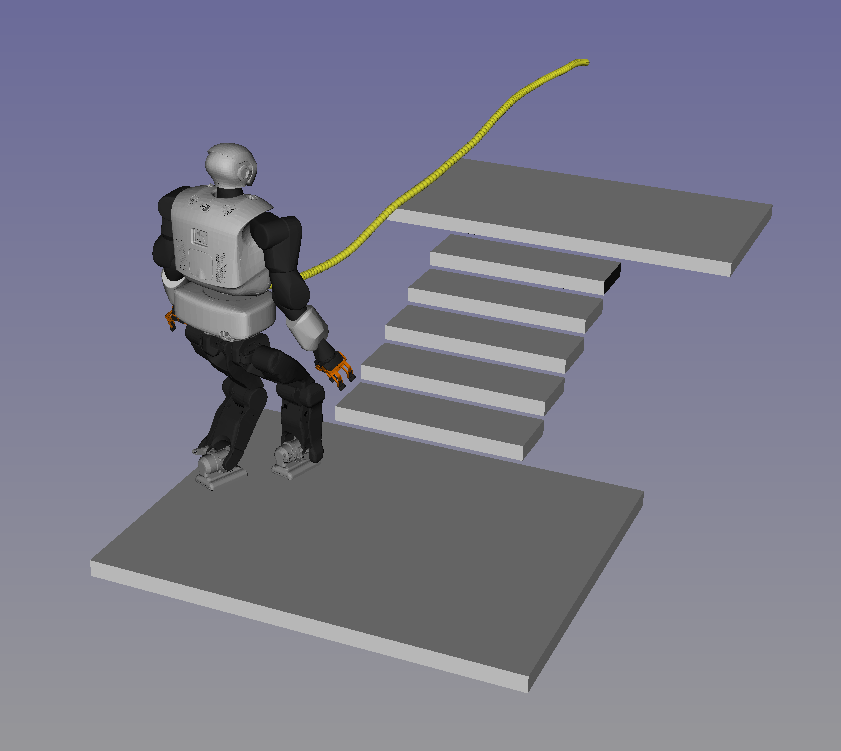
\includegraphics[width=0.8\textwidth, height=5cm]{Figures/Chapter_LEAS/stairs_exemple.png}
    \caption{Scene view}
    \end{subfigure}
    \begin{subfigure}[t]{0.49\linewidth}
    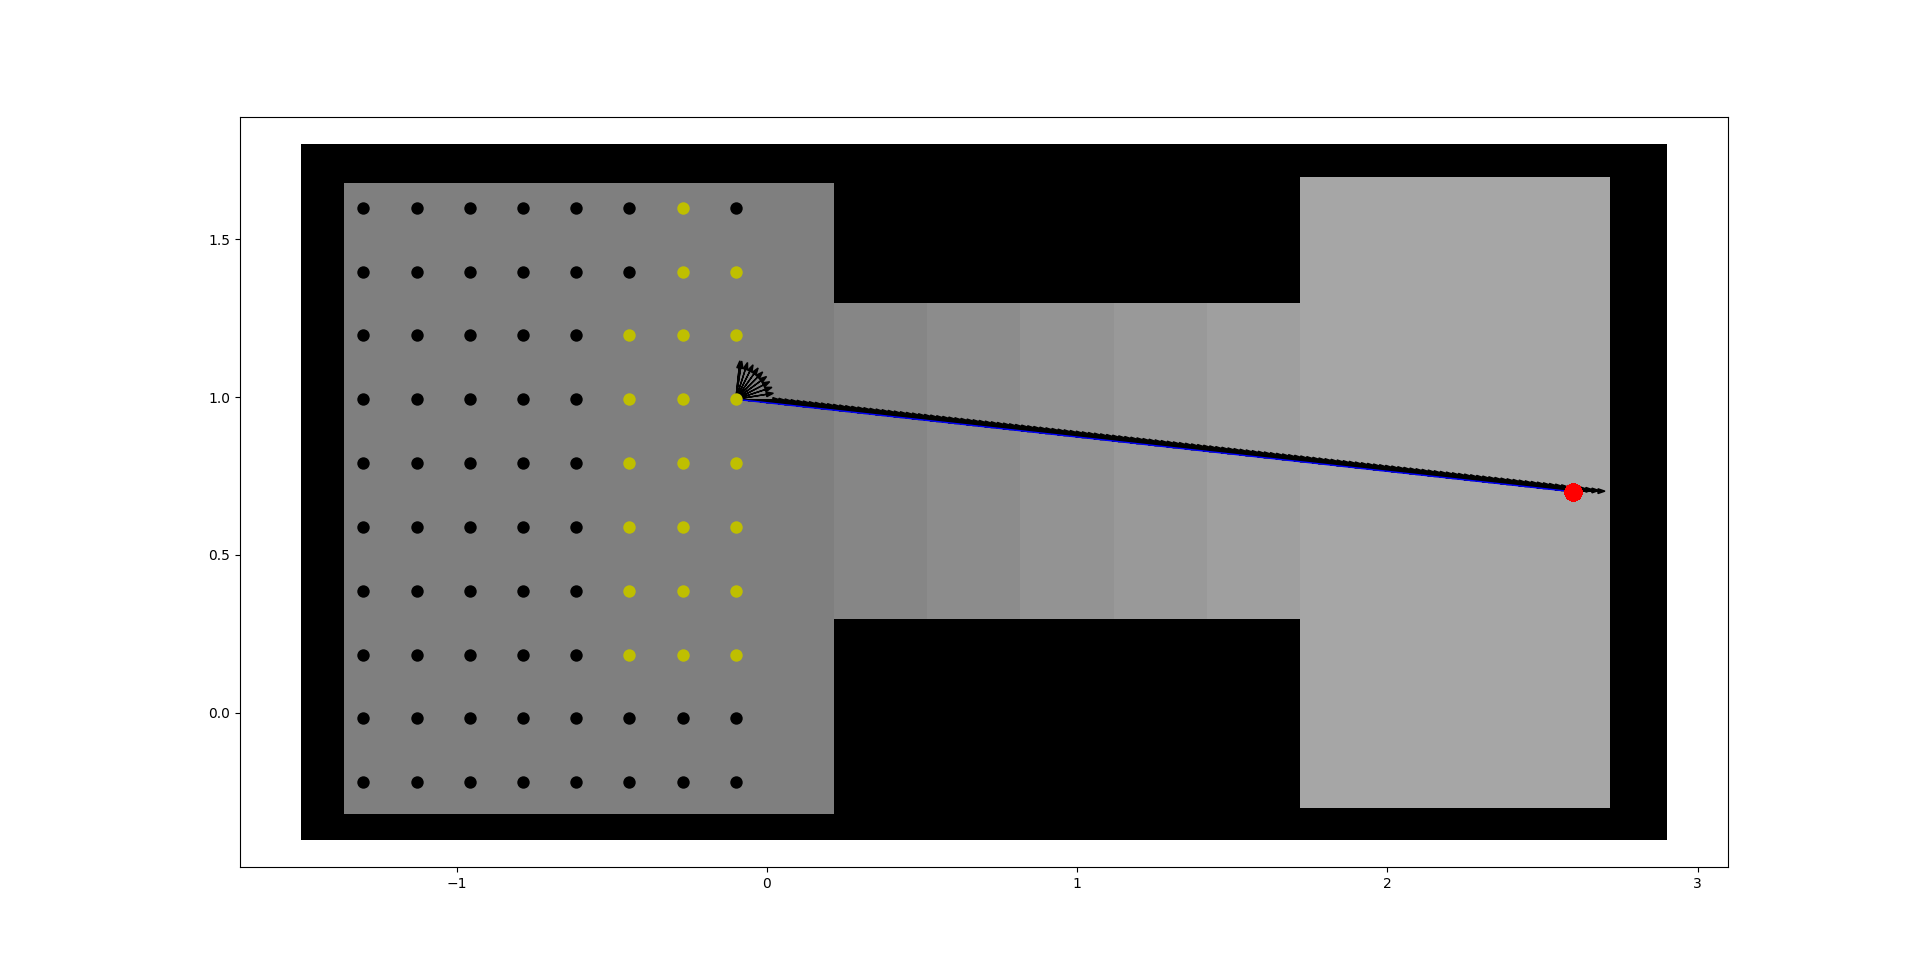
\includegraphics[width=\textwidth, height=5cm,trim={2cm 2cm 2cm 2cm},clip]{Figures/Chapter_LEAS/stairs_lin_p1_90.png}
    \caption{RB-Lin}
    \label{fig:leas:stairs_p1_lin}
    \end{subfigure}
    \begin{subfigure}[t]{0.49\linewidth}
    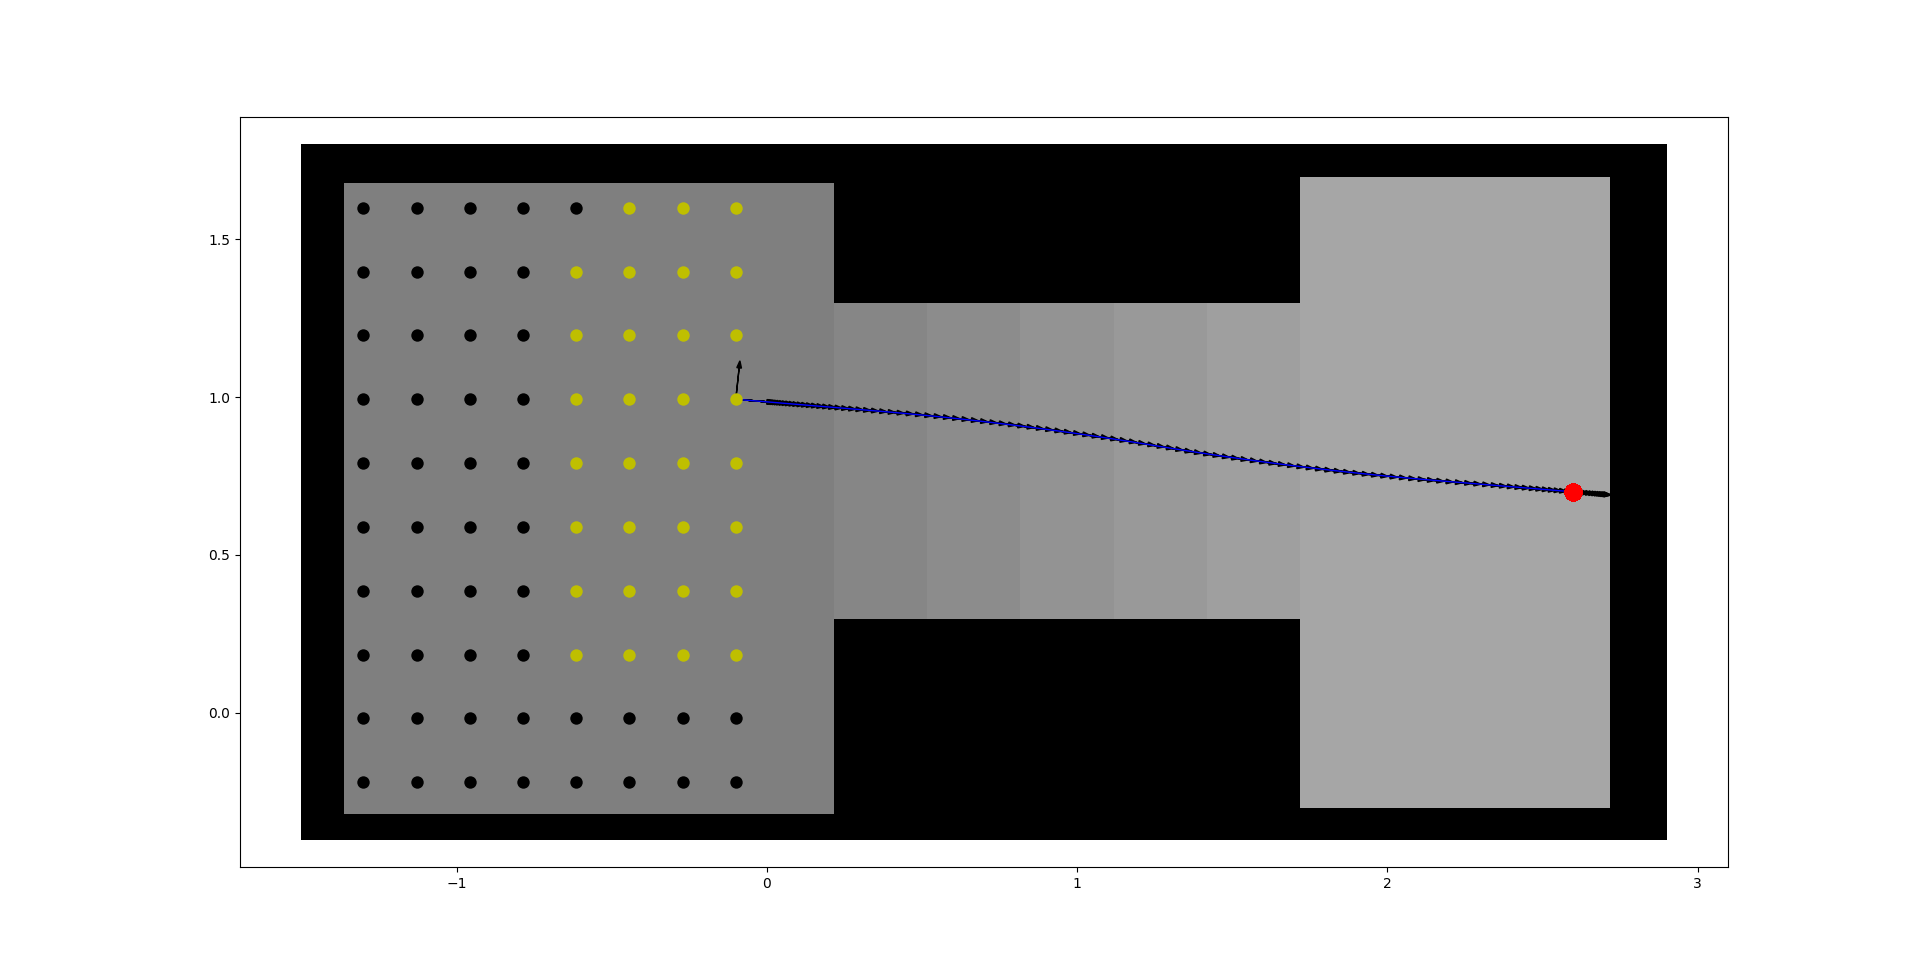
\includegraphics[width=\textwidth, height=5cm,trim={2cm 2cm 2cm 2cm},clip]{Figures/Chapter_LEAS/stairs_kino_p1_90.png}
    \caption{RB-Kino}
    \label{fig:leas:stairs_p1_kino}
    \end{subfigure}
    \begin{subfigure}[t]{0.49\linewidth}
    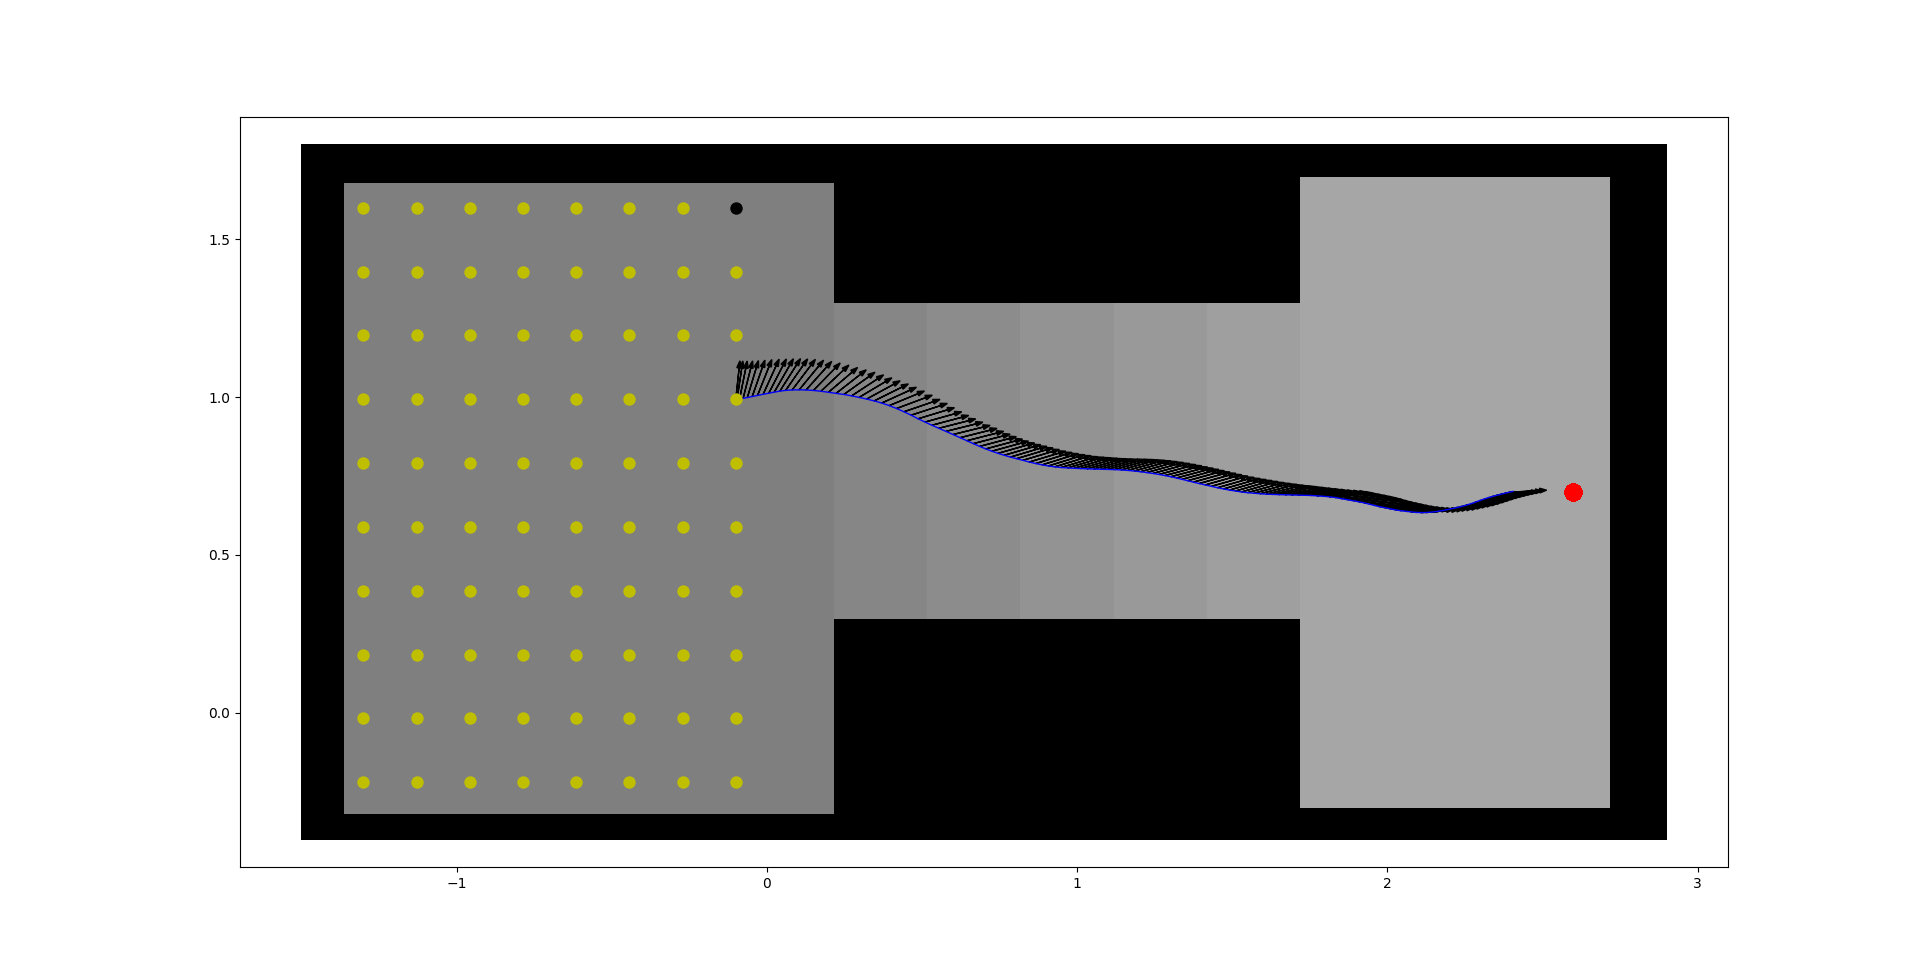
\includegraphics[width=\textwidth, height=5cm,trim={2cm 2cm 2cm 2cm},clip]{Figures/Chapter_LEAS/stairs_leas_p1_90.png}
    \caption{LEAS (ours)}
    \label{fig:leas:stairs_p1_leas}
    \end{subfigure}
    \caption{Comparison on stairs where dots represent initial states from where the SM generates a valid (yellow) or invalid (black) guide path up to the goal (red). We illustrate for each SM one trajectory where the black arrows represent the robot orientation along the guide.}
    \label{fig:stairs_p1}
\end{figure}

\hfill

\noindent\textbf{Stairs}. We compare the navigation skills of LEAS and our previous steering methods on the stairs scenario (Figure \ref{fig:stairs_p1}). The height map of the terrain is represented by the grey shades with the bottom of the stairs on the left, and the top of the stairs on the right. We uniformly sample 80 initial root configurations at the bottom of the stairs, from which the steering methods have to generate guide paths up to the same fixed goal location (red). Each initial state is oriented at $90^{\circ}$, to better show the rotation performed by the steering methods, and with a null velocity. 
Initial states from where the SM reaches the goal with a valid guide path are represented by yellow dots, and black dots represent states where either the SM fails to reach the goal or generates an invalid guide path (i.e. ground not reachable or collision) and thus requires path planning to succeed. 
For RB-Kino, we need to define additional constraints that are the velocity and acceleration desired on the goal configuration and that have an impact on the shape of the trajectory. In this scenario, we set both goal acceleration and velocity to $0$.

RB-Lin is designed to first rotate the robot toward the goal, then generate a straight line up to the goal (Figure \ref{fig:leas:stairs_p1_lin}). The main limitation of this method is that it succeeds only when directly placed in front of the stairs and further initial position on the left results in guide paths where the robot is unable to touch the ground.
RB-Kino presents the same limitation as RB-Lin, plus another one on the orientation where it rotates directly from $90^{\circ}$ to $0^{\circ}$ in one timestep (Figure \ref{fig:leas:stairs_p1_kino}). This is a problem inherent to RB-Kino which is the correlation between the initial velocity and the angular velocity. As a consequence starting with null velocity, as we will see later on, is critical with our contact planners as such fast rotation is not feasible kinematically. 
In practice, we avoid this problem by adopting the same strategy as RB-Lin by first rotating the robot to always start RB-Kino with a $0^{\circ}$ orientation.

LEAS  succeeds on a much broader range of initial states, hence removing the need for path planning in most cases (Figure \ref{fig:leas:stairs_p1_leas}). Our steering method generalizes to this scenario that has never been encountered during its training: it rotates and moves toward the goal, detects the stairs on its local height map, and adapts its velocity $v_z$ to climb it while keeping a valid state, finally reaching an area of $20$ cm around the goal.

% [2] On hole, compare with RB-Kino/RB-Lin, the picture with the points, success SM.
\hfill \break
\hfill \break

\begin{figure}[h]
    \centering
    \captionsetup[subfigure]{justification=centering}
    \begin{subfigure}[t]{0.4\linewidth}
    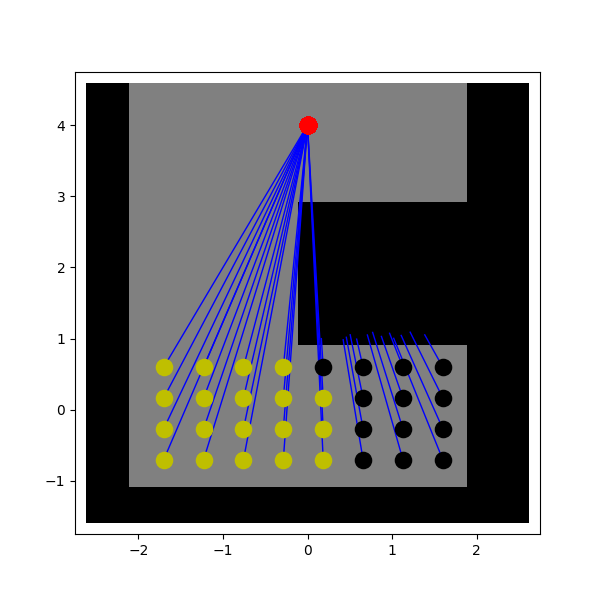
\includegraphics[width=\textwidth, height=4cm,trim={1cm 1cm 1cm 1cm},clip]{Figures/Chapter_LEAS/hole_p1_lin.png}
    \caption{RB-Lin}
    \label{fig:leas:hole:lin}
    \end{subfigure}
    \begin{subfigure}[t]{0.4\linewidth}
    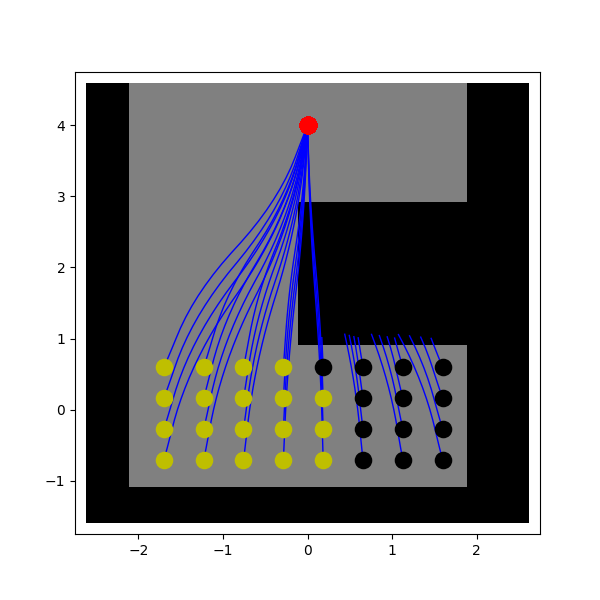
\includegraphics[width=\textwidth, height=4cm,trim={1cm 1cm 1cm 1cm},clip]{Figures/Chapter_LEAS/hole_p1_kino.png}
    \caption{RB-Kino}
    \label{fig:leas:hole:kino}
    \end{subfigure}
    \begin{subfigure}[t]{0.4\linewidth}
    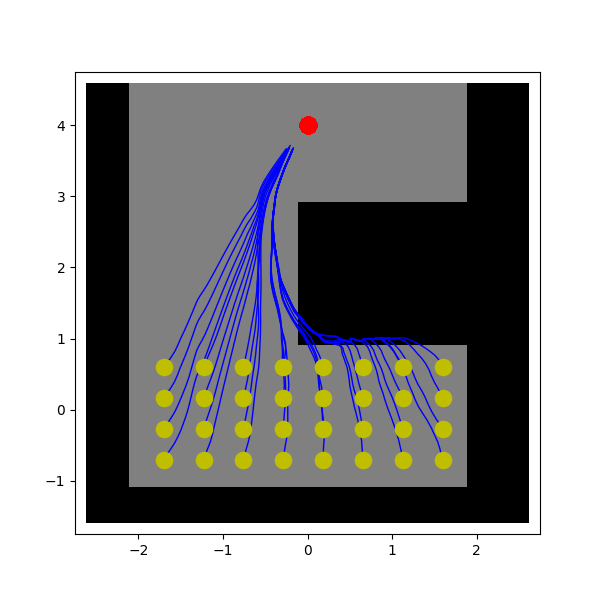
\includegraphics[width=\textwidth, height=4cm,trim={1cm 1cm 1cm 1cm},clip]{Figures/Chapter_LEAS/hole_p1_leas.png}
    \caption{LEAS (ours)}
    \label{fig:leas:hole:leas}
    \end{subfigure}
    \begin{subfigure}[t]{0.4\linewidth}
    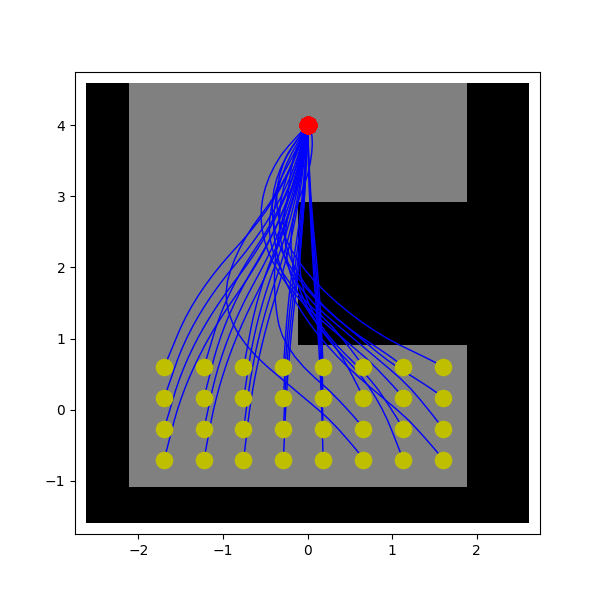
\includegraphics[width=\textwidth, height=4cm,trim={1cm 1cm 1cm 1cm},clip]{Figures/Chapter_LEAS/hole_p1_kino_rrt.png}
    \caption{RB-Kino + RRT}
    \label{fig:leas:hole_scenarios_Kino_RRT}
    \label{fig:leas:hole:kino_rrt}
    \end{subfigure}
    \caption{Comparison of steering methods on hole scenario where dots are initial states from where the SM generates a valid (yellow) or invalid guide path (black) invalid guide path up to the goal (red). Guide paths are represented by the blue trajectories.}
    \label{fig:leas:hole_scenarios}
\end{figure}

\noindent\textbf{Hole}. We now compare our steering methods on our hole scenario (Figure \ref{fig:leas:hole_scenarios}). Each initial configuration has a null velocity and is oriented toward the goal located on the other side of the hole. 
RB-Kino and RB-Lin generate valid guide paths only when the problem is feasible in a straight line and so require path planning for half of the initial configurations (Figures \ref{fig:leas:hole:lin} and \ref{fig:leas:hole:kino}).
In contrast, LEAS always succeeds in avoiding the hole and reaching the goal.
Even when starting from difficult configurations on the right, LEAS detects the hole and slowly slides along it while keeping a valid state.

% Still above the void
%We observe that some configurations still lie above the hole, less than 10 centimeters far from the surfaces. To fix this problem, a tighter constraint on the height map values under the robot can be set, as explained in Section \ref{subsub:validity_approximation}. %However, the Talos robot is 55 cm in width meaning that most of its body still lies above the ground.

%$\tilde{\mathcal{R}^*}$

% Hole kino and path planning
Finally, Figure \ref{fig:leas:hole_scenarios_Kino_RRT} illustrates RB-Kino combined with an RRT path planning algorithm to solve the hole scenario. The trajectories of (a,b,d) are generated using the full validity condition $\mathcal{R}$ without the stricter constraint (Section \ref{fig:approximation_validity}). Consequently, most guide paths generated lie above the hole with a maximum distance of $40$ cm from the surfaces, corresponding to the width of the range of motion of the Talos robot legs. 
This brings out the main problem of our previous validity condition $\mathcal{R}$ and the need to have a stricter constraint like $\tilde{\mathcal{R}^*}$ to avoid such configurations along the guide path.

%\textcolor{red}{TALK MORE ABOUT PATH PLANNING AND WHY WE DONT WANT TO USE IT HERE : 1.45s to compute it with bi-rrt on this scenario, several seconds on scenarios in their previous paper in C++. In comparison LEAS in python with my non-optimized code takes 0.56s in average on this scenario. => I can use the wall scenario to talk about that + need to add computation time on the hole scenario for Kino RRT}

% In general how much percent success in our scenarios ?
% -- On 1x11 with initial orientation of -180 degrees:
% Rubbles => 100/100
% Bridge => 31/100
% Stairs down => 100/100
% Stairs up => 86/100
% -- On 1x11 with initial orientation of 0 degrees:
% Rubbles => 100/100
% Bridge => 76/100
% Stairs down => 100/100
% Stairs up => 100/100

\hfill

\noindent\textbf{Evaluation of LEAS}. We evaluate the success of LEAS (Table \ref{tab:tests_1x11}) to navigate all the transition tiles of our evaluation terrain, never met during its training (Figure \ref{fig:tests_1x11}).
We uniformly sample 100 configurations before each transition tile with two different initial orientations, $0^{\circ}$ and $180^{\circ}$, to evaluate their impact on LEAS success. 


For both rubbles and stairs (down), LEAS succeeds in all 100 trajectories for both initial orientations. 
However, we observe some scenarios where our steering method fails, mainly from initial configurations facing backward and very close to the transition tile to cross. The agent thus fails to rotate the robot, to have a clear vision of the terrain type in its back, before navigating it. 
These difficult cases appear on the bridge where the agent stops the robot near the void to avoid falling, and on the stairs up where the agent collides with it during its rotation.
Despite these extreme cases, our steering method succeeds in crossing all the transition tiles of our scenario with a near $100$ \% success rate, hence demonstrating its terrain-aware navigation skills.

%Figure \ref{fig:leas_stop_void_obstacle} shows example scenarios where LEAS makes the robot idle to avoid unvalid configurations ($\mathcal{R}$ and $\mathcal{C}$).

Finally, we manually place some waypoints to reach a distant goal on a complex scenario as seen in Figure \ref{fig:bauzil_waypoints}. LEAS successfully reaches each waypoint navigating across this terrain composed of stairs and a bridge.

\begin{table}[h]
\centering
\begin{tabular}{ |c|c|c|c|c| } 
    \hline
    Initial orientation & Rubbles & Bridge & Stairs (down) & Stairs (up) \\ 
    \hline
    $0^{\circ}$ & 100 \% & 100 \% & 100 \% & 100 \%  \\ 
    \hline
    $180^{\circ}$ & 100 \% & 87 \% & 100 \% & 97 \% \\
    \hline
\end{tabular}
\caption{Success rate of LEAS For two initial orientations on 100 uniformly sampled trajectories for each transition tile (Figure \ref{fig:tests_1x11}). Initial positions can be far or near the transition tiles. LEAS needs enough time to rotate the robot, detect the transition tiles and navigate through it while keeping a valid configuration.}
\label{tab:tests_1x11}
\end{table}


\begin{figure}[h]
    \centering
    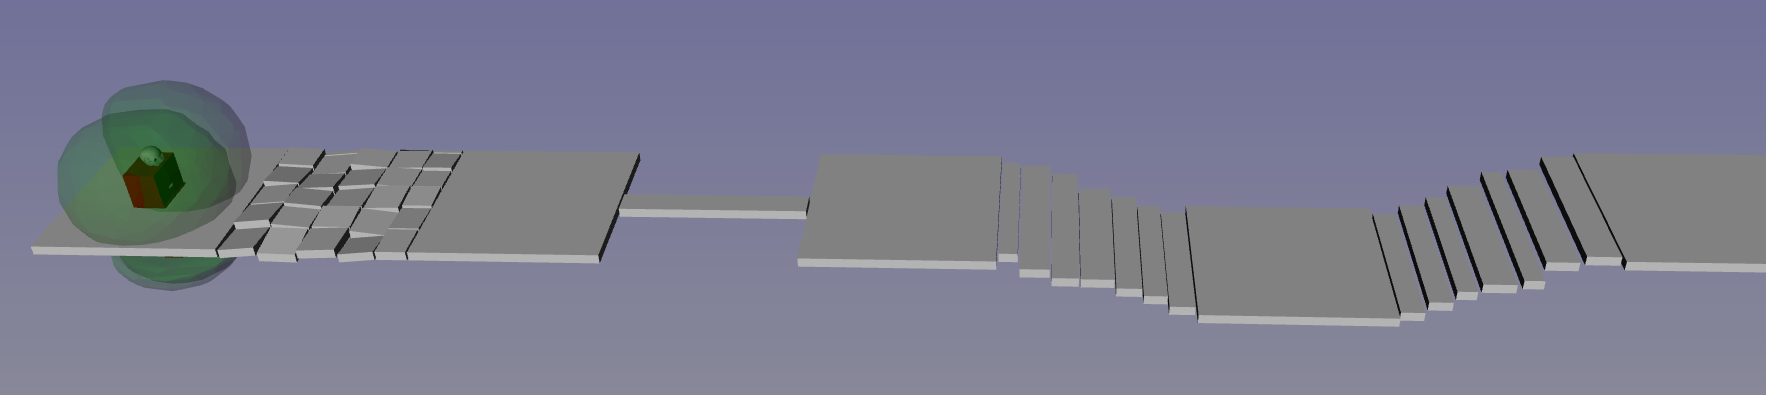
\includegraphics[width=0.8\textwidth,trim={0cm 0cm 0cm 0cm},clip, height=3.5cm]{Figures/Chapter_LEAS/1x11_tests.png}
    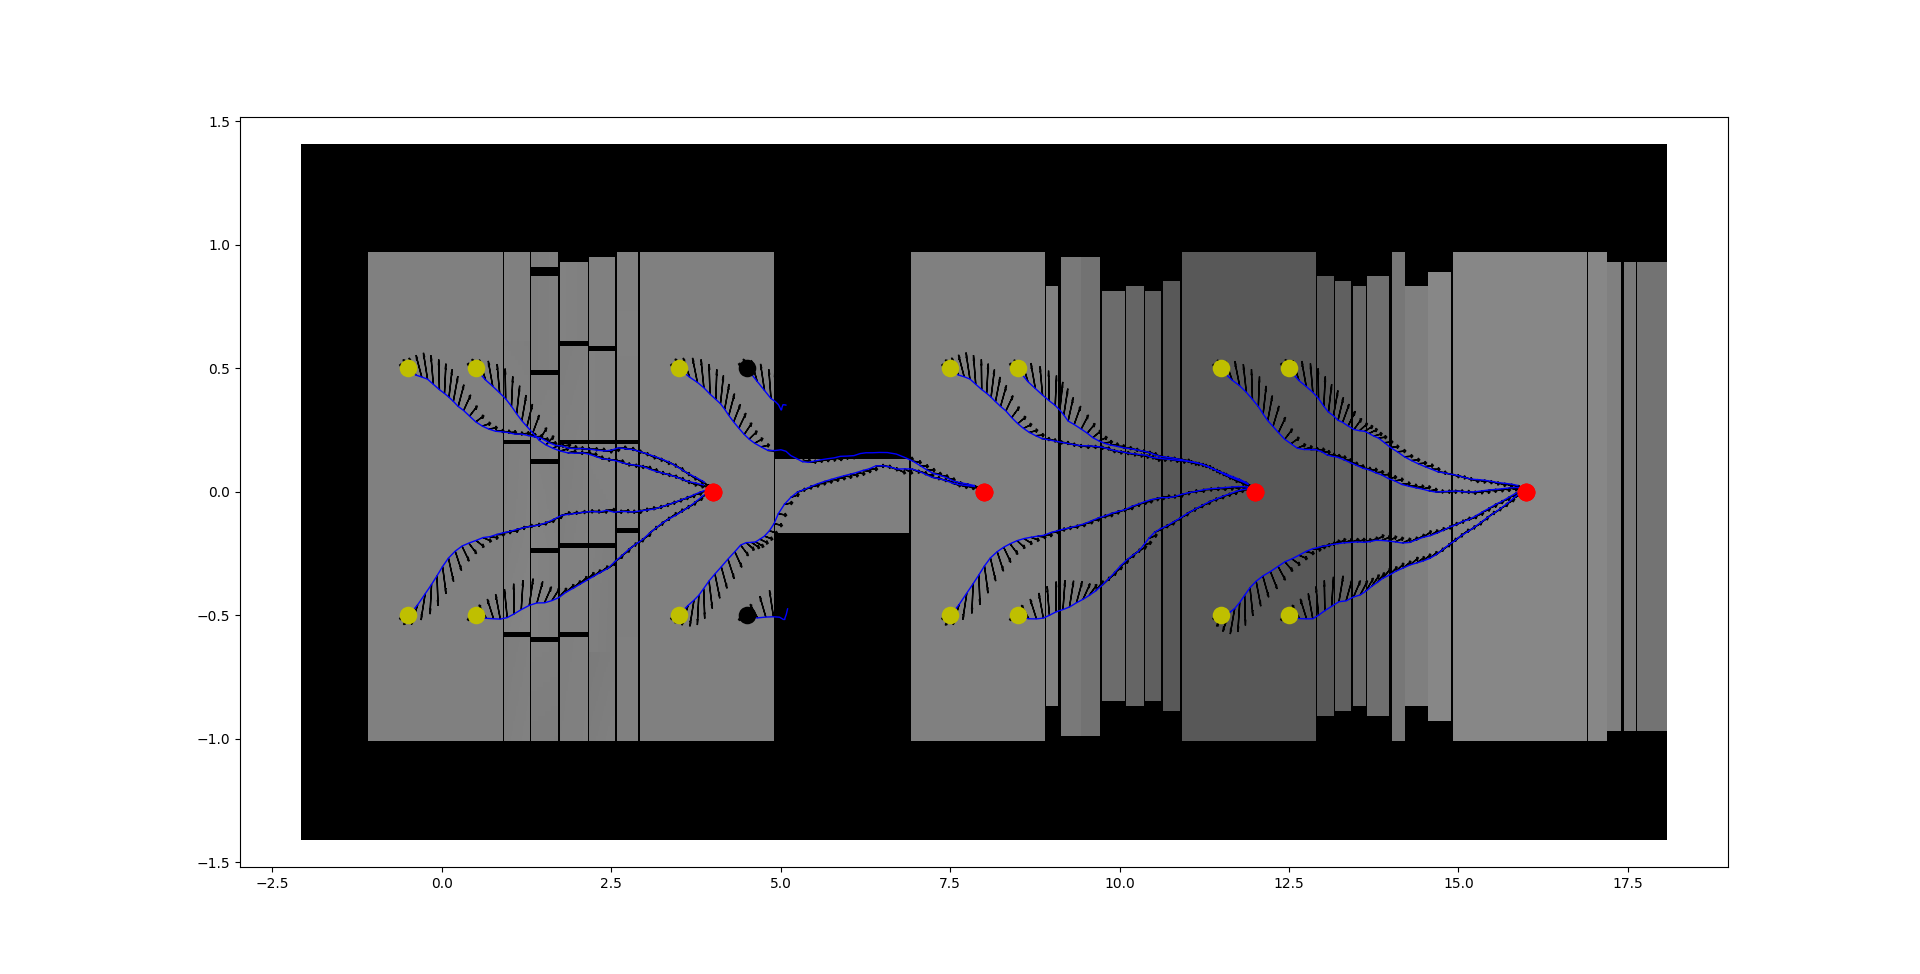
\includegraphics[width=\textwidth,trim={5cm 2cm 4cm 2cm},clip, height=6cm]{Figures/Chapter_LEAS/1x11_example_180deg.png}
    \caption{Evaluation terrrain with 4 transition tiles: rubbles, bridge, stairs (down), and stairs (up). Examples of extreme initial configurations (dots) from where LEAS generates: a valid (yellow) or invalid guide path (black) up to a goal (red). Black arrows are the root orientation along the guide (blue).}
    \label{fig:tests_1x11}
\end{figure}

% [1] Stop when there is an obstacle.
%\begin{figure}
%    \centering
%    \captionsetup[subfigure]{justification=centering}
%    \begin{subfigure}[t]{0.43\linewidth}
%    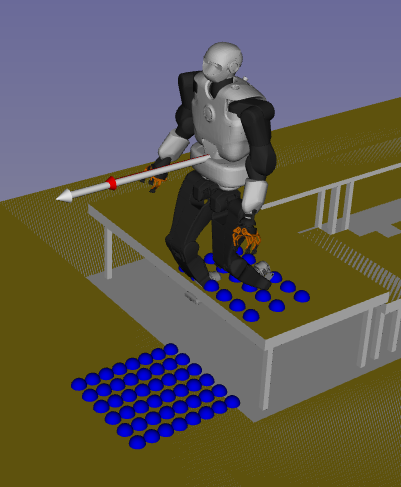
\includegraphics[width=\textwidth,height=6cm]{Figures/Chapter_LEAS/stop_bauzil_0.png}
%    \end{subfigure}
%    \begin{subfigure}[t]{0.43\linewidth}
%    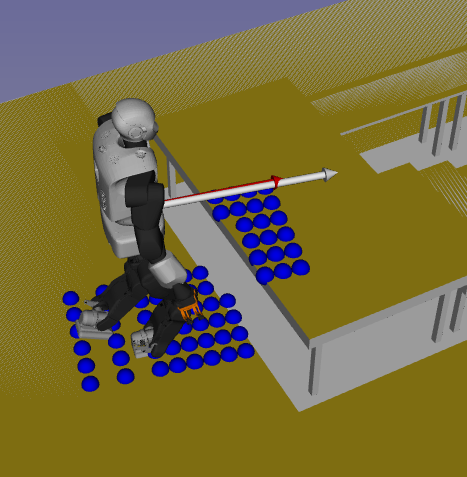
\includegraphics[width=\textwidth,height=6cm]{Figures/Chapter_LEAS/stop_bauzil_1.png}
%    \end{subfigure}
%    \label{fig:leas_stop_void_obstacle}
%    \caption{LEAS detects an obstacle and lower its velocity to avoid any unvalid state: collision or ground not reachable (robot contact configurations computed with SB-CP for a better visualization).}
%\end{figure}

\begin{figure}[t]
    \centering
    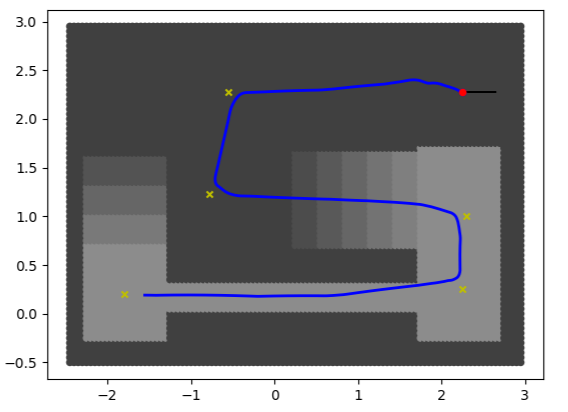
\includegraphics[width=0.6\textwidth, height=5cm]{Figures/Chapter_LEAS/follow_waypoints_bauzil.png}
    \caption{LEAS following manually placed waypoints (yellow cross) to reach a distant goal.}
    \label{fig:bauzil_waypoints}
\end{figure}




\section{Discussion\label{sub:leas:discussion}}
% Say that it works far better than before and offer a good compromise compared to our previous methods.
LEAS offers a flexible alternative to our previous steering methods. Our results show that LEAS performs better in generating valid guide paths, under collision-avoidance and reachability criteria, than RB-Kino and RB-Lin thanks to its local terrain awareness. 
This method learned by reinforcement succeeds in navigating all our test scenarios, while permitting a more flexible user control by providing a goal direction instead of a goal configuration. 
However, it also presents some limitations in its design and further improvements will be required in the future.

\subsection{Limitations}
% FAILURE CASES
% Fail often on the bridge
\noindent\textbf{Terrain visualization}.
Parameters $[z_{min}, z_{max}]$ as well as the height map resolution impacts the agent capabilities to detect its environment.
In our experiments, the most difficult scenarios to handle were navigating through bridges and obstacle avoidance, where the tuning of these values was critical.
First, a too high value $z_{min}$ can lead LEAS to interpret the void surrounding the bridge as a potential stair.
This caused LEAS to lower the robot root, at the limit of the collision with the trunk, to confirm if what it sees is a stair or a void. 
As a consequence, it can lead to some collisions with the bridge due to these two conflicting behaviors.
A similar problem appeared for a too low value $z_{max}$, with the interpretation of an obstacle as the next step of some stairs and causing a collision with it.
Finally, setting a too wide bound $[z_{min}, z_{max}]$ made the value of the heightmap difficult to interpret by our agent, that was unable to capture small to medium terrain variations.
The values we have selected offered a balanced trade-off, however, further tests are required to improve LEAS navigation performance.

% Play on R_ALIVE
To avoid such collisions, one could also increase $w_{alive}$ to encourage the robot to act more carefully. 
We tested this solution that greatly improved the LEAS capabilities for collision avoidance while keeping reachable states. However, LEAS was acting so safely that it did not dare to cross difficult transition tiles, thus making the robot idle in front of bridges to safely accumulate the reward $R_{alive}$. 
The final value $w_{alive}=1$ decided for LEAS offers a compromise safety/risk but requires further investigation. 

\hfill

% RL so the SM is not perfect and depends on many things
\noindent\textbf{Constraint on the orientation}. 
%Continuous agent learned by Reinforcement can still fail in performing their task, as LEAS due to a collision or staying idle instead of moving forward.
%An explanation of why the LEAS can present atypical behavior on some scenarios, why it does not succeed in generalizing or it generates guide path that are not straight is complex to analyze. It depends on the reward design, the control and the terrain where the agent has been trained on. 
% Exploration with orientation behaviour
We observed that LEAS trained on complex terrains tended to explore its surroundings by erratically orienting its root and so its local height map to have a better vision.
We limited this undesirable behavior by setting a high weight $w_{ori}$ to enforce its orientation toward the goal. 
However, such a reward will probably not work to navigate cluttered environments requiring the robot to sidewalk.

% Accuracy of LEAS
\begin{figure}
    \centering
    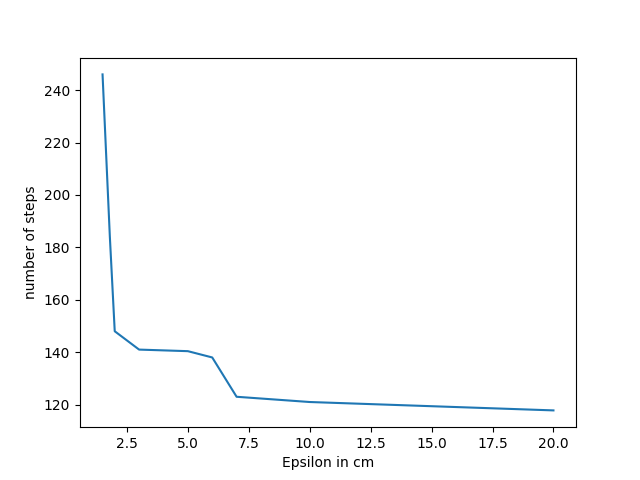
\includegraphics[width=0.6\textwidth, height=6cm]{Figures/Chapter_LEAS/test_epsilon.png}
    \caption{Average number of steps required to reach an area of radius $\epsilon$ cm around the goal.}
    \label{fig:nb_steps_required}
\end{figure}

\hfill

\noindent\textbf{Goal reaching accuracy}.
We recall one of the main limitations compared to our previous steering methods which is the non-exact connection to the goal position. We consider the goal as reached if the distance between the state on the guide path and the goal is inferior to a threshold of value $\epsilon$. In all our scenarios, we fix $\epsilon = 20$ cm that we consider accurate enough.
We further evaluate the accuracy of LEAS to reach a goal position in Figure \ref{fig:nb_steps_required}. For this test, we set the robot orientation back to the transition tile (rubbles for this scenario) and we uniformly sampled 50 configurations. The task to perform is to rotate the robot toward the fixed goal on the other side of the rubbles and get close to it, less than $\epsilon$ cm.
We test several values $\epsilon \in [1.5, 20]$ cm. 
For all $\epsilon \geq 1.5$ cm, all 50 trajectories reach the goal under the threshold. However, we can observe that as the value of epsilon decreases, the number of steps to reach the goal increases. Indeed, the agent passes close by the goal but misses the area of radius $\epsilon$ around it and has to move back and forth to reach such an accuracy. 
In this scenario, LEAS reaches the goal at once for all threshold $\geq 7.5 $ cm. In this thesis, we set $\epsilon=20$ cm to have a sufficient margin of error.

% Difficult to define good bounds for the height map to best represent small and high height variations. Using a second height map is a possibility but it increases the number of states and we want to avoid it. We could use a nonlinear, as a square function on values of the relative height map to better capture small variations near the robot's feet while ensuring height elevation detection for stairs, obstacles and void.
%\textbf{Surface detection}: 
\subsection{Future Improvements}

For a pure navigation task, LEAS without a contact planner does not need to clearly identify the surfaces of the terrain and solely focus on the reachability and collision conditions from the height map.
In this work we use a simple multilayer perceptron, as done in \cite{RL_RRT, RL_RRT_AUTORL} with 1-D lidar values, that is simple to implement and fast to train for our navigation task. 
However, we believe that LEAS could greatly benefit from convolutional neural network architectures to extract features from the height map and learn a better terrain representation \cite{deepLoco,deepGait,RLOC}.

The training terrain diversity was sufficient for LEAS to learn our navigation task, but more terrains could improve its generalization capabilities.
To do so, we could improve our terrain generator, or use another simulation environment such as RaiSim \cite{raisim} allowing us to efficiently switch between different terrains.

% How can we improve LEAS: As stated before, better terrains as grid terrains are still limited, biggers but with HPP not possible for now, more methods to have a better generalization with noise 
% + mirroring: it would be smart to mirror all the states and actions to generate twice as much datas. This would also get us a symmetric behaviour that we do not have for now.
%\textbf{Data augmentation}: 
Finally, we discussed using curriculum learning \cite{curriculum_learning_survey} to incrementally increase the complexity of the tasks to solve during the training, which did not improve the result of LEAS. But several methods in the literature could improve its learning efficiency and overall performance.
Especially mirroring all states relative to the robot orientation axis are other strategies to explore, that could greatly improve the sampling efficiency during the training and train a policy with a symmetric behavior.


\subsection{Conclusion}
% Recall that this is a prototype, but that is still better than our previous steering methods and in this paper we are aiming to see if a high level approach i.e. with a guide path can improve the performances of the contact planners.
% Conclusion
We presented LEAS, an RL steering method to locally navigate complex terrains and to generate guide paths subject to reachability and collision avoidance constraints. 
Such terrain-aware steering methods remove the need for a path planning algorithm, expensive to compute, in most of our basic scenarios.
As a result, LEAS can directly be integrated as the module P1 of our locomotion pipeline (Figure \ref{fig:pipeline}).

Yet, we did not solve the feasibility problem between our navigation task ($P1$) and the contact planner ($P2$), and that is why in the next chapters we answer the following question: 
\textit{can LEAS navigate complex terrains while generating feasible guide paths by a given contact planner?}